% !TEX encoding = UTF-8 Unicode
% !TEX spellcheck = en-US

%%===================================

\documentclass[10pt,b5paper]{report}
\usepackage{styles/thesisstyle}

%%===================================

% glossaries must be defined in the preamble
%\usepackage[acronym,toc]{glossaries}
%\makeglossaries
%\newglossaryentry{latex}
{
    name=latex,
    description={Is a mark up language specially suited for scientific documents}
}

\newglossaryentry{maths}
{
    name=mathematics,
    description={Mathematics is what mathematicians do}
}

\newglossaryentry{formula}
{
    name=formula,
    description={A mathematical expression}
}

\newacronym{gcd}{GCD}{Greatest Common Divisor}

\newacronym{lcm}{LCM}{Least Common Multiple}

\begin{document}

%%%%%%%%%%%%%%%%%%%%%%%%%%%%%%%%%%%%%%%%
% titlepage
% !TEX encoding = UTF-8 Unicode
%!TEX root = main.tex
% !TEX spellcheck = en-US

%This is the Titlepage
%%=========================================
\thispagestyle{empty}

\begin{center}

\includegraphics{fig/NTNU}
\end{center}

\mbox{}\\[5.5pc]
\begin{center}
\Large\textbf{\Proxc{} -- A CSP\hyp{}inspired Concurrency Library for Modern \Cpp{} with Dynamic Multithreading for Multicore Architectures}\\[2pc]

\Large{Edvard Severin Pettersen}\\[1pc]
\large{Trondheim June 2017}\\[2pc]

MASTER THESIS TTK4900\\
Department of Engineering Cybernetics\\
Norwegian University of Science and Technology
\end{center}
\vfill

\noindent Supervisor: Professor Sverre Hendseth

\noindent Co-supervisor: Øyvind Teig

\afterpage{\blankpage}

 
% !TEX encoding = UTF-8 Unicode
%!TEX root = main.tex
% !TEX spellcheck = en-US
%%=========================================
\setcounter{page}{0}
\pagenumbering{arabic}
\newpage
\phantomsection
\section*{Project Description}
\label{sec:project_description}

Create a concurrency framework for \Cpp{}, based on abstractions of Communicating Sequential Processes (CSP). The focus of this framework should be the utilization of multicore architectures. Present a design and implementation of such framework, and discuss limitations and uses.

\begin{flushleft}
Assignment given: 01. january, 2017\\
Supervisor: Sverre Hendseth, ITK
\end{flushleft}


\afterpage{\blankpage}


\setcounter{page}{0}
\pagenumbering{roman}

%%%%%%%%%%%%%%%%%%%%%%%%%%%%%%%%%%%%%%%%
% pre-content
% !TEX encoding = UTF-8 Unicode
%!TEX root = main.tex
% !TEX spellcheck = en-US
%%=========================================

\newpage
\phantomsection
\section*{Preface}
\addcontentsline{toc}{section}{Preface}


\begin{flushright}
\texttt{Edvard Severin Pettersen}\\

\includegraphics[width=0.3\linewidth,right]{fig/signature}
Trondheim, 2017-06-04
\end{flushright}

\afterpage{\blankpage}

% !TEX encoding = UTF-8 Unicode
%!TEX root = main.tex
% !TEX spellcheck = en-US
%%=========================================

\newpage
\phantomsection
\section*{Abstract}
\addcontentsline{toc}{section}{Abstract}

This thesis presents the work done on ProXC++: a CSP\hyp{}inspired concurrency library for C++. ProXC++ emphasizes on dynamic multithreading, allowing to create high\hyp{}performance multiprogrammed systems for multicore architectures. The thesis argues the motivation for a dynamic multithreaded library is necessary for fully utilize the available resources in the future of multicore processors. A design and implementation of ProXC++ is presented, as well as giving examples of usage on how to use the library. A set of tests with various degrees of parallelism are benchmarked with ProXC++ against other similiar multithreaded CSP frameworks, as well as their singlecore equivalent implementations. The results from the benchmarks are promising, indicating ProXC++ are fully capable of utilizing the available resources in most cases. However, a slight issue with the distribution of large scale parallel work with ProXC++ is highlighted and discussed. Limitations and uses of ProXC++ is discusses, and a list of potential future work is presented. Lastly, a conclusion is drawn.

\vfill

\afterpage{\blankpage}

% !TEX encoding = UTF-8 Unicode
%!TEX root = main.tex
% !TEX spellcheck = en-US
%%=========================================

\newpage

\begingroup
\makeatletter
% Redefine the \chapter* header macro to remove vertical space
\def\@makeschapterhead#1{%
  %\vspace*{50\p@}% Remove the vertical space
  {\parindent \z@ \raggedright
    \normalfont
    \interlinepenalty\@M
    \Huge \bfseries  #1\par\nobreak
    \vskip 15\p@
  }}
\makeatother

\tableofcontents
\endgroup

\afterpage{\blankpage}


\setcounter{page}{0}
\pagenumbering{arabic}

%%%%%%%%%%%%%%%%%%%%%%%%%%%%%%%%%%%%%%%%
% introduction
% !TEX encoding = UTF-8 Unicode
%!TEX root = main.tex
% !TEX spellcheck = en-US
%%=========================================

%%%%%%%%%%%%%%%%%%%%%%%%%%%%%%%%%%%%%%%%%%%%%%%%%%%%%%%%%%%%%%%%%%%%%%%%%%%%%%%%
\chapter{Introduction}
\label{ch:introduction}


In this day and age, multicore processors seems to have been the next big step in processor evol\-ution. Ever since singlecore processors hit the physical limitations of Moore's law, it was no longer sustainable to \textit{just} increase the number of transistors and clock frequency in a processor. This is of course an oversimplification of the issue, but the transition to multicore processors is very much real, as well as the amount of research currently going into multicore processors.


Back in the days when developing software, an often viable strategy when performance was not adequate was to wait for faster and more performant hardware. This mainly relied on sequential software scaling in performance with the increase in performance of singlecore processors. With multicore processors, this strategy is no longer feasible. Software needs to be developed with more efficient utilization of processor resources, and scalability of said resources. 


Concurrent programming is the main tool for programmers to develop such software. Even though concurrent programming has existed long before multicore became the predominant architecture, it forms the foundation allowing software to take advantage of this parallel processing capability. Concurrent programming is a great way to model and implement systems which are inherently parallel, as it introduces powerful concepts for expressing such parallel compositions in software. However it also introduces new potential challenges which could cause unwanted behaviour.


Communicating Sequential Processes (CSP) was an effort by Tony Hoare to harness the expressiveness of concurrent programming while being able to prove the correctness of such models. CSP is not programming language, but a formal language used to describe concurrent systems. These systems are described by a concurrent composition of sequential processes, which only communicate through message-passing.


Several programming languages (occam-$\pi$, Go, XC) exists which incorporate the CSP formalism to various degrees, but the mainstream popularity has not been great; Go is an exception, which ranks as one of the most popular languages to date. As a response to this lack of mainstream popularity, a collection of libraries and transpilers have been created to offer the CSP formalism to better established languages and platforms. This includes languages such as C++, Python, Java, and more. 


As a lack of a modern CSP library for C and C++, the library ProXC was created as an attempt to fill this void. ProXC was based on user-threads, with no support for multicore. This allowed for fairly simple design of the runtime system, including the scheduler, channel, and alternation. ProXC gave promising results compared to what Go and occam achieved on a singlecore, but was not able to provide a multicore design nor implementation. A multicore design and implementation of such library could potentially be beneficial for utilizing the vast resources of multicore processors which currently exists. 

This report introduces ProXC++, a concurrency library for C++. ProXC++ offers many of the same features ProXC provides, however ProXC++ provides multicore support acheived through dynamic multithreading. ProXC++ is written in C++14. The design and implementation of ProXC++ is presented in this report, examples on how ProXC++ can be used, and how it performs compared to existing languages and libraries. Further on, limitations and uses is discussed, as well as future work. A conclussion is drawn.  blah blah blah.


\section{Project Status of ProXC}


\section{Thesis Structure}

%%%%%%%%%%%%%%%%%%%%%%%%%%%%%%%%%%%%%%%%
\part{Preliminaries} \label{part:preliminaries}

% !TEX encoding = UTF-8 Unicode
%!TEX root = main.tex
% !TEX spellcheck = en-US
%%=========================================


%%%%%%%%%%%%%%%%%%%%%%%%%%%%%%%%%%%%%%%%%%%%%%%%%%%%%%%%%%%%%%%%%%%%%%%%%%%%%%%%
\chapter{Background}
\label{ch:background}


In this chapter a more in-depth explanation of different topics mentioned in the introduction, as well as other relevant topics, is presented. These topics cover the required background knowledge for the project, as well as existing programming languages and libraries that shows some equivalence to this project. Each topic is presented on its own, and how it relates to this project. 


%%%%%%%%%%%%%%%%%%%%%%%%%%%%%%%%%%%%%%%%%%%%%%%%%%%%%%%%%%%%%%%%%%%%%%%%%%%%%%%%
\section{Concurrent Programming}
\label{sec:concurrent_programming}
% threads, semaphores, mutexes, monitors, atomic operations
% deadlocks, livelocks, starvation


Concurrent programming, or concurrent computing, is a form of computing to express programs or systems which execute multiple sequential computations in interleaving time periods. These computations are said to be running \textit{concurrently}, compared to \textit{sequentially} (one completing before the next start). These computations are often called \textit{processes} or \textit{threads}, which indicate an individual, separate execution point. 

The notion of concurrency stems from the limitations of sequential programs and how all programs in the end is translated to machine code. Given the program is executed on a uniprocessor, only one machine code instruction will be executed at any given time\footnote{Machine code execution is vastly more complex then presented here, e.g. pipelining and instruction-level parallelism (ILP), but the sequential nature of program execution still stands}.  Since all computations in a sequential program must be executed sequential, it can be unintuitive how to model and implement concurrent systems which does not easily translate to sequential systems. Concurrency aims to provide an abstraction level to bridge this limitation. Concurrent systems are therefore much more expressive than sequential systems, since it does not matter whether the program is executed in parallel or not, e.g. on a multiprocessor or uniprocessor.

It is important to note that concurrent programming is not the same as parallel programming. Concurrency is a form of abstraction, disregarding how the actual program execution is achieved. Parallelism refers to, in contrast to concurrency, the condition of a program being executed on multiple processors at once. One could therefore say that concurrency is possible on both uniprocessors and multiprocessors, while parallelism is only possible on multiprocessors.

Concurrency is a great tool for programmers, allowing expressing concurrent systems in a much more intuitive manner. It does however introduce a much greater mental overhead for the programmer, and is much more error prone compared to other types of programming paradigms. As a result, concurrent programming may not be as easy to invest time in. FIXME


%%%%%%%%%%%%%%%%%%%%%%%%%%%%%%%%%%%%%%%%
\subsection{Threading Models}
\label{subsec:threading_models}

Threading is the foundation of concurrency, which allows multiple computations to be executed simultaneously. Some sort of threading mechanism must be implemented on the platform to provide concurrency. On \textit{operating systems} (OS), threading mechanisms mainly falls into three types of threading models: \textit{user-threads}, \textit{kernel-threads}, or \textit{hybrid-threads}, which is a combination of the two first models. \citet{c++csp2} goes into further detail on the three models, and a short summary is presented below.


\subsubsection{User-Threading}

User-threads are a cooperative scheduling of threads executed in user space\footnote{Regarding operating systems is a set of locations where normal user processes run}, and is called a \texttt{M:1} threading model. \texttt{M:1} means running \texttt{M} user-threads on a single kernel-thread. These user-threads must cooperate on scheduling, as the scheduling is non-preemptive\footnote{Running task is executed until completion or yields}. Context switching and scheduling between these user-threads is happening unbeknownst to the OS, resulting in much faster context switch times. This does however mean the OS cannot help with scheduling, and blocking calls in any user-thread blocks all user-threads on the given kernel-thread. Only one user-thread can run on a kernel-thread at any time.


\subsubsection{Kernel-Threading}

Kernel-threads are often directly supported in OS kernels and is called a \texttt{1:1} threading model. \texttt{1:1} means scheduling each kernel-thread onto the available processors of the system. Kernel-threads often use preemptive scheduling\footnote{Tasks are given a priority, and the running task is interrupted and later resumed whenever a task with higher priority is ready}, which the OS is responsible for. Kernel-threads has no problems with blocking calls, as the OS can schedule any other kernel-thread during a blocking call. Since the OS has full control over the scheduling it can more better utilize the available resources and time usage for each thread, compared to user-threading. Context switching is however much slower than user-threads because of overhead and kernel-space\footnote{Regarding operating systems is the location where the code of the kernel is stored and executed} crossing.


\subsubsection{Hybrid-Threading}

Hybrid-threads is a combination of user-threads and kernel-threads, and is called a \texttt{M:N} threading model. \texttt{M:N} means running \texttt{M} user-threads on \texttt{N} kernel-threads. In other words, hybrid-threading runs multiple kernel-threads, with each kernel-thread running multiple user-threads. Blocking calls can still cause issues with unnecessarily blocking user-threads, but is possible to mitigate with running the blocking user-thread on its own kernel-thread. Scheduling the user-threads among the kernel-threads can be much more difficult compared to user-threading, as the OS cannot help with utilizing the available resources. 


%%%%%%%%%%%%%%%%%%%%%%%%%%%%%%%%%%%%%%%%
\subsection{Concepts and Primitives}
\label{subsec:concepts_primitives}

Having multiple sequential executions running concurrently is not very useful if they cannot cooperate. Some form of interaction or communication between the computations, which in turn requires coordination of access to shared resources, must therefore be present. This coordination is called \textit{concurrency control}. Concurrency control means ensuring the correct and intended result from concurrent interactions are upheld. 

To be able to manipulate shared resources safely requires introducing couple of new primitives and concepts. Below is a non-exhaustive list of concurrency primitives presented.


\subsubsection{Atomic Operations}

An operation is said to be \textit{atomic} or \textit{linearizable} if it appears to the rest of the system as instantaneous. In concurrent systems multiple processes can access the same shared resource at the same time. If one of the processes are changing the contents of a shared resource while another process is using the same resource, it is possible the operation results in an invalid or undefined state. It is obvious such situations requires atomic operations to force a linear sequence of well\hyp{}defined observable operations. 

Atomic operations exists both as low level and high level primitives. At the bottom we have processor instructions which are used to manipulate memory atomically. These might include \textit{atomic read / write}, \textit{atomic swap}, \textit{test\hyp{}and\hyp{}set}, \textit{fetch\hyp{}and\hyp{}add}, \textit{compare\hyp{}and\hyp{}swap}, and \textit{load\hyp{}link / store\hyp{}conditional}. Modern processors usually support these types of instructions FIXME(CITE). Further, these instructions are used to implement higher level primitives such as locking and lock\hyp{}free and wait\hyp{}free algorithms. 


\subsubsection{Critical Sections}

Concurrent access to shared resources can result in an invalid or undefined state, as stated above. If more than one processes in a region where shared resources are accessed can cause erroneous behaviour, than such regions are called a \textit{critical sections} or \textit{critical regions}. These regions must therefore be protected by some sort of synchronization or lock mechanism. Critical sections usually accesses shared resources such as a data structure, IO operations or network socket, where multiple concurrent access would result in incorrect behaviour \citep{raynal2012concurrent}.

Consider the following program: two processes, \texttt{A} and \texttt{B}, tries to increment the shared resource \texttt{count} by one. 

\noindent\begin{minipage}{0.45\textwidth}
\begin{lstlisting}[title={Process A},style={CustomC},frame={},xleftmargin={4em}]
// Critical section
count = count + 1
\end{lstlisting}
\end{minipage}
\begin{minipage}{0.45\textwidth}
\begin{lstlisting}[title={Process B},style={CustomC},frame={},xleftmargin={4em}]
// Critical section
count = count + 1
\end{lstlisting}
\end{minipage}

If both process \texttt{A} and \texttt{B} are executing the critical section at the same time, it is possible for the \texttt{count} resource to only be incremented once, instead of the expected result twice. This comes from the fact to incrementing is not inherently an atomic operation, but a three\hyp{}stage operation of read\hyp{}modify\hyp{}write. 

If process \texttt{A} starts executing the increment, but is preempted before the write stage, process \texttt{B} can theoretically complete an arbitrary amount of increment operations before process \texttt{A} is resumed again. When process \texttt{A} is resumed, the old modified value of \texttt{count} is now written back instead of the updated value. This is a classic example of a \textit{race condition}, meaning the order of which the operation is completed determines the outcome.

To achieve correct behaviour the critical section must be protected, usually done through some form of mutual exclusion. This consequently makes the critical section an atomic operation, as the read\hyp{}modify\hyp{}write operation is made indivisible to the other process.


\subsubsection{Semaphores}

Semaphore is in software terms a data structure used to control access to a shared resource between multiple processes and to synchronize between processes. Invented by Edsger Dijkstra \citep{dijkstra}, and is one the simplest concurrency primitives used to build concurrency structures.

As described in \citet[chapter 2]{downey2016}, a semaphore is like an integer with three differences:

\begin{enumerate}[topsep=0em,itemsep=-1em,partopsep=0.5em,parsep=1em]
    \item When you create the semaphore, you can initialize its value to any integer, but after that the only operations you are allowed to perform are increment (increase by one) and decrement (decrease by one). You cannot read the current value of the semaphore.
    \item When a thread decrements the semaphore, if the result is negative, the thread blocks itself and cannot continue until another thread increments the semaphore.
    \item When a thread increments the semaphore, if there are other threads waiting, one of the waiting threads gets unblocked.
\end{enumerate}

Blocking in this sense means the scheduler will suspend the blocking thread until a corresponding event or operation which causes the thread to be unblocked. 

Both the increment and decrement operations are atomic, meaning multiple processes can concurrently access a semaphore.

Semaphores usually comes in two flavours: \textit{counting semaphore} and \textit{binary semaphore}. A counting semaphore allows an arbitrary resource count, while a binary semaphore allows only resource count of $0$ and $1$ (hence binary). 

Semaphores is incredibly simple by definition, and are therefore often used to create more complex concurrency synchronization and structures. This includes structures such as \textit{locks}, \textit{monitors} and other \textit{synchronization patterns}. See \citet[chap. 3-7]{downey2016} for a more complete overview of such constructs.


\subsubsection{Mutual Exclusion (Mutex)}

Mutual exclusion, \textit{mutex} for short, is necessary for protecting critical regions from concurrent access and to prevent race conditions. One can view mutexes as binary semaphores, with one important difference: mutexes has a notion of ownership. Only the process which is successful in acquiring the mutex can release it. 

Looking back at the example in ``Critical Sections'', wrapping a mutex around the critical section hinders process \texttt{A} and \texttt{B} to increment \texttt{count} simultaneously, and effectively turns the increment operation into an atomic operation. 

\noindent\begin{minipage}{0.45\textwidth}
\begin{lstlisting}[title={Process A},style={CustomC},frame={},xleftmargin={4em}]
mutex.wait()
// Critical section
count = count + 1
mutex.signal()
\end{lstlisting}
\end{minipage}
\begin{minipage}{0.45\textwidth}
\begin{lstlisting}[title={Process B},style={CustomC},frame={},xleftmargin={4em}]
mutex.wait()
// Critical section
count = count + 1
mutex.signal()
\end{lstlisting}
\end{minipage}

Note that using mutual exclusion is very error prone, and might have unwanted side\hyp{}effects and conditions such as deadlocks, starvation and priority inversion. This is explained in further detail in the next subsection.


%%%%%%%%%%%%%%%%%%%%%%%%%%%%%%%%%%%%%%%%
\subsection{Potential Problems}
\label{subsec:potential_problems}

As a consequence of using concurrency control, potential problems such as \textit{race conditions}, \textit{deadlocks}, \textit{livelocks}, \textit{starvation}, and \textit{priority inversion} must be taken into consideration. These are unwanted conditions or program states which are results of concurrent operations and interactions which resulted in an erroneous state.


\subsubsection{Race Condition}

As mentioned before, race condition is when the output of an operation is dependent on the timing and sequence of other processes. Race conditions is never an intended behaviour of a program, as it is deemed undefined behaviour. This comes from the fact that the result is of a race condition is the non\hyp{}deterministic result of timing between threads. 


\subsubsection{Deadlock}

Deadlocks is a state in which a group of processes are each waiting for other members of the same group to release a lock, effectively halting progression. This is a direct consequence of enforcing mutual exclusion in critical sections.

As described in \citet[page 239]{silberschatz2006operating}, a deadlock can only occur in a system if and only if all four of the \textit{Coffman conditions}\citep[First described][page 70]{coffman1971system} are held simultaneously. The conditions are as follows:

\begin{enumerate}[topsep=0em,itemsep=-1em,partopsep=0.5em,parsep=1em]
    \item \textit{Mutual exclusion} -- the resources involved must be unshareable.
    \item \textit{Hold and wait} -- a process holding at least one resource and requesting additional resources.
    \item \textit{No preemption} -- a resource can only be voluntarily released by the process holding it.
    \item \textit{Circular wait} -- each process must be waiting for a resource held by another process, which in turn is waiting for the first process to release the resource.
\end{enumerate}

There are several ways to handle deadlocks, but the three main approaches are \textit{ignoring}, \textit{detection} and \textit{prevention}. Ignoring is simply to assume a deadlock never occurs. Detection allows deadlocks to occur. If a deadlock is detected, the deadlock symmetry is broken by either terminating one or more of the deadlocked processes, or involuntarily preempt one or more of the deadlocked resources. Prevention is to simply prevent one of the four Coffman conditions from ever occurring.


\subsubsection{Livelock}

Livelock is similar to deadlock, as it is a state in which processes are not blocked, but are refrained from making progression. This can occur when processes are to busy responding to each other to resume work. 

Livelock is a rarer condition than deadlock, and can be harder to detect as the processes are not blocked when livelocked. 


\subsubsection{Starvation}

Starvation is a condition where a process is denied further progress by perpetually denied access to required resources or denied running time by higher priority processes. 

The absence of starvation in concurrent algorithms is called \textit{liveness}, which is a property guaranteeing all processes being able to make progress within finite time. 


\subsubsection{Priority Inversion}

Priority inversion is a situation in scheduling where a higher priority process is indirectly preempted by a lower priority process, usually because of mutual exclusion. 

Consider the following example: process \texttt{H}, \texttt{M} and \texttt{L} has the priority ordering \texttt{p(H) > p(M) > p(L)}, and \texttt{H} and \texttt{L} both try to acquire the resource \texttt{R}. If \texttt{L} acquires the resource and is promptly preempted by \texttt{H}, \texttt{H} becomes blocked until \texttt{L} releases the resource. It is now possible for \texttt{M} to run over \texttt{L}, because of higher priority. Effectively \texttt{H} cannot run as \texttt{L} cannot release the resource, since \texttt{M} is preempting \texttt{L}. This is called \textit{priority inversion}.

\textit{Bounded priority inversion} is when it can be proven priority inversion only occurs for a finite amount of time, while \textit{unbounded priority inversion} cannot prove this. 



%%%%%%%%%%%%%%%%%%%%%%%%%%%%%%%%%%%%%%%%%%%%%%%%%%%%%%%%%%%%%%%%%%%%%%%%%%%%%%%%
\section{Communicating Sequential Processes}
\label{sec:csp}
% what is CSP
% programming languages
% libraries

\textit{Communicating sequential processes} (CSP) is a mathematical formal language used in computer science to describe and model concurrent systems. First introduced by \citet{hoare1978communicating}, and was originally described as parallel composition of sequential disjoint processes with primitives for input and output, combined with guarded commands \citep{dijkstra1975guarded}. Communication was solely through message\hyp{}passing, which permitted synchronized communication between named processes.

Since its inception, CSP has undergone numerous transformations. As \citet{abdallah2005communicating} explains, most of the subsequent research has focused on a process algebra known as \textit{Theoretical CSP} (TCSP), which suppresses the imperative aspect of CSP \citep{brookes1984theory}. 

The strong points of CSP and TCSP is the ability to reason about correctness of the system being modeled. Since all communication between processes are limited to message\hyp{}passing, no primitive race conditions can occur. Further on, properties of the CSP models can be reasoned about, such as liveness, safety and deadlock. 

In the industry, CSP is used to specify and verify the correctness of concurrent systems, especially communication and security protocols. The most prominent tool used is the \textit{failure\hyp{}divergence refinement} (FDR) checker \citep{manual2000failures}. FDR can statically prove if a concurrent system refines a given specification, has the correct liveness and safety properties, as well as absence of deadlocks and divergence. It is obvious such tools are powerful for systems that must prove its correctness before being deployed.

The ideas and expressiveness of CSP models has influenced the creation of concurrent programming languages, most notable occam \citep{inmos1988occam}, Ada \citep{ledgard1983reference}, XC \citep{douglas2009programming} and Go \citep{go2009go}. CSP frameworks has also been developed for programming languages which does not natively support CSP influenced concurrency, such as ProXC \citep{pettersen2016proxc} for C, C++CSP2 \citep{brown2007c++csp2} and CPPCSP \citep{chalmers2016cppcsp} for C++, JCSP \citep{welch2007jcsp} for Java, PyCSP \citep{bjorndalen2007pycsp} for Python, and much more.

It is understandable CSP is a great tool for concurrent systems. It provides a strong and safe framework for modelling and implementation, and allowing to prove the correctness of an implementation. This alleviates some of the mental overhead, as well as reducing the error prone nature of concurrent programming. 


%%%%%%%%%%%%%%%%%%%%%%%%%%%%%%%%%%%%%%%%%%%%%%%%%%%%%%%%%%%%%%%%%%%%%%%%%%%%%%%%
\section{Multicore Architectures}
\label{sec:multicore_architectures}
%caches
%parallelism

FIXME, necessary to write about this?


%%%%%%%%%%%%%%%%%%%%%%%%%%%%%%%%%%%%%%%%%%%%%%%%%%%%%%%%%%%%%%%%%%%%%%%%%%%%%%%%
\section{Memory Ordering}
\label{sec:memory_ordering}
% weak vs. strong
% relaxed, acquire, release, seq_cst

Out of all CPU operations, memory accesses are among the slowest. Following Moore's law, CPU instruction performance has increased at a much greater rate than memory performance. Use of multilevel caches has been used to a great extent to bridge this gap in performance, however utilization of said caches could be improved. This is where \textit{memory reordering} comes in. To increase the performance of memory access further and properly utilize the hardware parallelism, memory operations can complete out of order \citep{mckenney2007memory}.

Several types of memory\hyp{}consistency models exist. \textit{Sequential consistency} is a guarantee that all processes agree on the order memory operations occur, even if they are completed out of order. The easiest configuration for sequential consistency is running all processes on a single core or a uniprocessor architecture. On multicore or multiprocessor architectures however, memory reordering can create inconsistencies between processes and proper care must therefore be taken to enforce correct memory ordering. 

There are different types of memory reordering, which usually falls into the categories of \textit{compiler reordering} and \textit{processor reordering}. As the name implies, compiler reordering is memory reordering done by the compiler at compile time, while processor reordering is memory reordering done by the processor at runtime.

Compiler reordering is obviously different from compiler to compiler, as it is implementation defined for each compiler. Processor reordering is also surprisingly different from CPU to CPU architecture. A \textit{memory model} is therefore used to describe what types of memory ordering to expect at runtime for a given processor, which again falls into the two categories \textit{weak} and \textit{strong} memory models.

As \citet{preshing2012weakstrong} explains it, a weak memory model can expect all types of memory reordering. This means any load or store operation can be reordered with any other load or store operation, and can reordered by both the compiler or processor. In contrast, a strong memory model limits the types of memory reordering. More specifically, only \texttt{store\hyp{}load} reordering is permitted. 

To enforce correct memory ordering, some type of \textit{memory barrier} must be used \citep{preshing2012barriers,preshing2012lockfree}. These exists as both software and hardware semantics, and are generally implemented as some sort of \textit{acquire} and \textit{release} semantics \citep{preshing2012acquire}.


%%%%%%%%%%%%%%%%%%%%%%%%%%%%%%%%%%%%%%%%%%%%%%%%%%%%%%%%%%%%%%%%%%%%%%%%%%%%%%%%
\section{Non\hyp{}Blocking Algorithms}
\label{sec:nonblocking_algorithms}
% wait-free and lock-free programming

To fully utilize multiprocessors, most programs are multiprogrammed. Preemptive multiprocessor operating systems has the unfortunate effect of degrading performance in synchronized parallel programs if the preemption is ill\hyp{}timed, and access to shared data structures is usually the root of the cause. As \citet{michael1998nonblocking} explains, these data structures needs to ensure concurrent access is consistent and well\hyp{}formed across processes, which is usually implemented by protecting critical sections with mutual exclusion. Mutual exclusion locks does not scale well in performance on time\hyp{}sliced multiprogrammed systems \citep{zahorjan1991effect} due to preemption of processes holding locks. The preempted process must be rescheduled and release the lock before any waiting processes can progress.

One principal strategy to mitigate ill\hyp{}timed preemptions are \textit{non\hyp{}blocking algorithms}. Non\hyp{}blocking algorithms has the property any process cannot cause failure nor suspension of any other process, despite failures or suspension of itself. Two types of guarantees are usually associated with nonblocking algorithms to describe how strong this property is: \textit{lock\hyp{}free} and \textit{wait\hyp{}free}. 

Lock\hyp{}freedom guarantees system\hyp{}wide progress, and can be defined as: given a meaningful definition of progress, an algorithm is lock\hyp{}free if at least one process in a program makes progress if all processes are given sufficient running time. Wait\hyp{}freedom guarantees process\hyp{}wide progress, and can be defined as: an algorithm is wait\hyp{}free if every operation in the algorithm has an upper bound of computational time before it completes. Wait\hyp{}freedom implies lock\hyp{}freedom, which makes wait\hyp{}freedom a stronger guarantee than lock\hyp{}freedom.

\citet{preshing2012lockfree} describes the \textit{lock} part of non\hyp{}blocking algorithms (or as lock\hyp{}free programming he refers it to) as ``the possibility of "locking up" the entire application in some way, wheth\-er it's deadlock, livelock -- or even due to hypothetical thread scheduling decisions made by your worst enemy''. This means code not containing locks, such as mutexes, may still not be lock\hyp{}free. 

It is rare a concurrent program is entirely lock\hyp{}free or wait\hyp{}free, which is why the focus is on non\hyp{}blocking algorithms rather than non\hyp{}blocking programs. Generally, a set of high contention operations in programs are set out to be non\hyp{}blocking, such as access and manipulation to shared data structures.

A handful of techniques are used to implement non\hyp{}blocking algorithms, most commonly a combination of atomic operations, memory barriers and general patterns. While the atomic primitives \texttt{read\hyp{}modify\hyp{}write} and \texttt{compare\hyp{}and\hyp{}swap} forms the basis of most non\hyp{}blocking algorithms, memory models and memory ordering needs to be taken into consideration as well. Since different processors have different memory models, it is not given processes agree on the order in which memory operations occur. Memory reordering can cause memory inconsistencies between processes, which is why sequential consistency or memory barriers are needed, especially on multicore architectures \citep{preshing2012weakstrong,preshing2012barriers,preshing2012lockfree,preshing2012acquire}.


%%%%%%%%%%%%%%%%%%%%%%%%%%%%%%%%%%%%%%%%%%%%%%%%%%%%%%%%%%%%%%%%%%%%%%%%%%%%%%%%
\section{Dynamic Multithreading}
\label{sec:dynamic_multithreading}
% work stealing and work sharing

Getting the potential performance out of multicore processors requires fully utilizing the available cores. Amdahl's law \citep{amdahl1967validity} argues that the maximum potential speedup in a program with infinite number of parallel processors is limited to $^1/_s$, given the fraction of sequential work in the program is $s$. Because of Ahmdal's law, multiprogrammed concurrent programs needs to identify the potential parallelism and convert sequential work into parallel work to exploit multicore performance. This responsibility is mostly up to the programmer to identify, and in most cases is easier said than done. Simple constructs such as loops and loosely coupled sections are easy to detect and convert \citep{dagum1998openmp,robison2013composable}, but a program\hyp{}wide parallelism is far from intuitive to detect and how to schedule such parallelism effectively on multicore processors. 

\textit{Dynamic multithreading} is a strategy to abstract away the scheduling and instead focus on detecting the units of parallel work in the program. The idea is letting the program create, synchronize and schedule new processes or tasks which executes some kind of computation. 

Based on the threading models (see \cref{subsec:threading_models}) the naïve approach is spawning kernel\hyp{}threads for each process. The operating system is responsible for creating, scheduling and destroying the processes, as well as scheduling the processes among the available cores. However, kernel\hyp{}threads are expensive to create, context switching between kernel\hyp{}threads are relative slow, and scales very badly in performance with an increase in kernel\hyp{}threads running simultaneously. This severely limits the use of processes, and makes it very unintuitive on how to distribute the parallel work efficiently.

Using hybrid\hyp{}threads, a combination of user\hyp{}threads running on multiple kernel\hyp{}threads, is an improvement on only kernel\hyp{}threads. Each spawned process is a user\hyp{}thread, scheduled on a static number of kernel\hyp{}threads equal to the number of available cores. User\hyp{}threads are much cheaper to create, context switching is relatively much faster, and scales performance wise much better. The problem is how to efficiently schedule and distribute these processes between the available kernel\hyp{}threads, since an intermediate runtime environment has to exist between the user\hyp{}threads and the operating system.

Two principal scheduling strategies exist to efficiently distribute and schedule processes among a static number of kernel\hyp{}threads, namely \textit{work stealing} and \textit{work sharing}.


%%%%%%%%%%%%%%%%%%%%%%%%%%%%%%%%%%%%%%%%
\subsection{Work Stealing}
\label{subsec:work_stealing}

Given a processor with $P$ cores, $P$ kernel\hyp{}threads are created with each running a scheduler. Each scheduler has a pool of ready work. Whenever a schedule runs out of ready work, it selects another scheduler (called victim) and tries to steal work. If the steal was successful, it continues the stolen work. Spawning processes simply pushes the spawned process in the ready pool \citep{blumofe1999scheduling}.

Different types of work stealing algorithms exist, but the main emphasis is on the victim selection and stealing procedure. The most popular algorithm is the randomized work stealing algorithm first detailed in \citet{blumofe1999scheduling}. Whenever a scheduler is empty for ready work, a victim is chosen uniformly at random. If the victims ready pool is not empty, try to steal work. If successful, resume said work, else start over the selection procedure.

The most common way to represent ready work is by using a double\hyp{}ended queue, or \textit{deque} for short, where the ends of the deque is called \textit{top} and \textit{bottom}. The scheduler owning the deque has access to the bottom of the deque, where it can push and pop ready work. Any other schedulers can try to steal from the top of the deque if it is non\hyp{}empty. Much research has gone into creating these deques as efficient and low overhead as possible \citep{chase2005dynamic,le2013correct}, as they can be high contention area between kernel\hyp{}threads.

Many runtime frameworks for dynamic parallel computations has been created with work stealing \citep{blumofe1996cilk,sunderam1990pvm}, and with great success performance wise.


%%%%%%%%%%%%%%%%%%%%%%%%%%%%%%%%%%%%%%%%
\subsection{Work Sharing}
\label{subsec:work_sharing}

As the same setup as work stealing, $P$ kernel\hyp{}threads are created on a processor with $P$ cores with each running a scheduler. The big contrast to work stealing is work sharing manually distributes each work among the schedulers whenever new work is spawned. 

Usually work stealing is preferred over work sharing, as work stealing causes less process migration between schedulers. As \citet[page 721]{blumofe1999scheduling} argues, ``Intuitively, the migration of threads occurs less frequently with work stealing than with work sharing, since when all processors have work to do, no threads are migrated by a work stealing scheduler, but threads are always migrated by a work sharing scheduler''.


% !TEX encoding = UTF-8 Unicode
%!TEX root = main.tex
% !TEX spellcheck = en-US
%%=========================================


%%%%%%%%%%%%%%%%%%%%%%%%%%%%%%%%%%%%%%%%%%%%%%%%%%%%%%%%%%%%%%%%%%%%%%%%%%%%%%%%
\chapter{CSP + Multicore = True ?}
\label{ch:multicore_csp}


This chapter takes the motivation described in the introduction and elaborates on why a multicore CSP library would be desirable. Further, a review of existing solutions of multicore CSP programming languages and libraries is presented and how they work.


%%%%%%%%%%%%%%%%%%%%%%%%%%%%%%%%%%%%%%%%%%%%%%%%%%%%%%%%%%%%%%%%%%%%%%%%%%%%%%%%
\section{Motivation behind Multicore CSP}
\label{sec:multicore_csp_motivation}


As mentioned in the introduction, software can no longer rely on increase in processor performance for an increase in software performance. High performance software which wishes to utilize the full potential of multicore processors needs to do two things: identify the parallel units of work in a program, and efficiently run the parallel work using the available processor resources. 

Why is it important to identify parallel units of work in a program? The short answer is Amdalh's law \citep{amdahl1967validity}. Amdalh's law argues the maximum speedup in a program with infinite number of parallel processors is limited to $^1/_s$, given the fraction of sequential work in the program is $s$. If a program has a fraction of $50\%$ sequential work the maximum speedup possible is $2$, and a fraction of $25\%$ sequential work yields a maximum speedup possible of $4$. There exists more refined models of Amdalh's law developed for different multicore architectures \citep{sun2010reevaluating}, but the point is the same; parallelism is key.

If a programmer cannot reduce the fraction of sequential work, or in other words cannot increase the fraction of parallel work, there is not much to gain from multicore processors. Increasing the fraction of parallel work usually consists of identifying parallelism in sequential work, and subsequently converting said work to parallel units of work. Identifying parallelism is usually the easiest part, e.g. loops and decoupled sections of code are easy to identify and reason whether is parallel or not. How to convert sequential work to parallel work is however another matter, requiring details of scheduling and synchronization.

When parallel work has been identified, how do you efficiently schedule and run the parallel work on the available processor resources? When you want the program to be scalable for all multicore processors, simply hard coding for a given multicore architecture will not suffice. Dynamic multithreading is a solution, which has strategies for dynamically distribute parallel work among available processor cores. Strategies include work stealing and work sharing, but the core philosophy is letting the dynamic multithreading take care of scheduling and synchronization, while the programmer specifies what the parallel work is. Whether dynamic multithreading is implemented with the program or as part of a runtime system underneath achieves the same goal. 

This thesis argues CSP is a good candidate for creating high performance software for multicore processors. First of all, CSP provides expressive and safe abstractions for creating concurrent systems, which also can be statically reasoned whether certain specifications and safety properties are met. Secondly, CSP inherently defines its parallel units of work, as all CSP models are a parallel composition of sequential processes. This inherent parallel nature of CSP essentially identifies all higher level units of parallel work in a program. Now, if a dynamic multithreading scheme was employed together with a CSP framework, it would enable exploiting the parallel nature of multicore processors.


%%%%%%%%%%%%%%%%%%%%%%%%%%%%%%%%%%%%%%%%%%%%%%%%%%%%%%%%%%%%%%%%%%%%%%%%%%%%%%%%
\section{Existing Solutions of Dynamic Multithreaded CSP}
\label{sec:multicore_csp_existing}


Combining CSP with dynamic multithreading is no new invention. Even tough dynamic multithreading has usually not been the focus with CSP framework, multiple frameworks does exists with dynamic multithreading, including programming languages and programming libraries. The frameworks varies in availability and age, ranging from proprietary programming languages to open\hyp{}source libraries. Below is a non\hyp{}exhaustive list of dynamic multithreaded CSP frameworks summarized.


%%%%%%%%%%%%%%%%%%%%%%%%%%%%%%%%%%%%%%%%
\subsection{Programming Languages}


Not many programming languages has made concurrency a native part of the language design, yet alone CSP\hyp{}based concurrency. For those languages with CSP as a native influence, dynamic multithreading has usually not been the focus. The first CSP\hyp{}based languages was designed for microprocessor hardware, and with the years transitioned to general\hyp{}purpose programming languages. Below are the three most influential CSP\hyp{}based programming languages with dynamic multithreading presented.


\subsubsection{occam on the Transputer}


\subsubsection{XC on XMOS}


\subsubsection{Go}


%%%%%%%%%%%%%%%%%%%%%%%%%%%%%%%%%%%%%%%%
\subsection{Programming Libraries}


Several CSP\hyp{}based concurrency libraries has been developed for more popular and established programming languages not supporting CSP natively. Below are the most influential CSP\hyp{}based concurrency libraries with dynamic multithreading presented.


\subsubsection{C++CSP2}


\subsubsection{C++CSP}


\subsubsection{Boost.Fiber}



%%%%%%%%%%%%%%%%%%%%%%%%%%%%%%%%%%%%%%%%
\part{ProXC++ -- The Library} \label{part:proxc++}

% !TEX encoding = UTF-8 Unicode
%!TEX root = main.tex
% !TEX spellcheck = en-US
%%=========================================

%%%%%%%%%%%%%%%%%%%%%%%%%%%%%%%%%%%%%%%%%%%%%%%%%%%%%%%%%%%%%%%%%%%%%%%%%%%%%%%%
\chapter{Library Specifications}
\label{ch:library_specifications}

This chapter introduces the library developed for this thesis. Details regarding design and implementation are presented in \cref{ch:design_implementation}


%%%%%%%%%%%%%%%%%%%%%%%%%%%%%%%%%%%%%%%%%%%%%%%%%%%%%%%%%%%%%%%%%%%%%%%%%%%%%%%%
\section{Library Overview}
\label{sec:library_overview}
% API
% features

ProXC++ (pronounced ``proxy plus plus'') is a CSP\hyp{}influenced concurrency library for modern C++, specifically aimed at dynamic multithreading for multiprogrammed parallel programs. Modern C++ in this regard meaning support for C++14 standard and later. The central ambition of ProXC++ is to provide expressive and safe concurrency to C++ programs which fully and effectively utilizes available computational resources on multicore architectures.

ProXC++ is a runtime system using a hybrid threading model. Work stealing is employed for load balancing between the schedulers, each running on an available logical core. 

Available concurrency primitives in ProXC++ are \textit{fork\hyp{}and\hyp{}join} parallelism, strict message\hyp{}passing, simultaneous event handling, and soft real\hyp{}time requirements.

The name ``ProXC++'' is a continuation of the original library ProXC \citep{pettersen2016proxc}, where ProXC++ targets C++ in contrast to ProXC targeting C. Since ProXC++ aimed to be an improvement over ProXC, the ``\textit{plus plus}'' could also be viewed as an ``\textit{incremental better}'' library. This is of course only intended to be humorous, as I personally like ``\textit{plus plus}'' better than slapping a ``2'' at the end of the name.


%%%%%%%%%%%%%%%%%%%%%%%%%%%%%%%%%%%%%%%%%%%%%%%%%%%%%%%%%%%%%%%%%%%%%%%%%%%%%%%%
\section{Library Features}
\label{sec:library_features}

The complete set of features in ProXC++ is as follows:

\begin{itemize}[topsep=0em,itemsep=-1em,partopsep=0.5em,parsep=1em]
    \item Multicore support
    \item Lightweight processes / threads
    \item Unidirectional, type\hyp{}safe, one\hyp{}to\hyp{}one synchronous channels
    \item Parallel; fork\hyp{}and\hyp{}join parallelism on a set of processes
    \item Replicators for parallel, generating dynamic number of parallel processes
    \item Alternation; choice over multiple alternatives
    \item Alternatives of types channel read, channel write, and timeouts on timers
    \item Alternatives guarded on a boolean value
    \item Replicators for alternation, generating dynamic number of choices
    \item Timers; types of relative, repeating, and absolute timeouts
    \item Soft real\hyp{}time requirements for process suspension, channel operations, and alternation operations
\end{itemize}


%%%%%%%%%%%%%%%%%%%%%%%%%%%%%%%%%%%%%%%%%%%%%%%%%%%%%%%%%%%%%%%%%%%%%%%%%%%%%%%%
\section{Target Platforms}
\label{sec:target_platforms}

ProXC++ is mainly targeted for desktop environments, especially multicore architectures. However, it should support all platforms that has access to a C++14 compliant compiler and the Boost C++ libraries \citep{boost2017boost} as well as the Boost Context library \citep{kowalke2017boost} (as Boost is portable). ``\textit{Should}'' is used here, because ProXC++ is only tested on 64\hyp{}bit x86 Linux platform as of writing this thesis.


%%%%%%%%%%%%%%%%%%%%%%%%%%%%%%%%%%%%%%%%%%%%%%%%%%%%%%%%%%%%%%%%%%%%%%%%%%%%%%%%
\section{Dependencies}
\label{sec:dependencies}

ProXC++ uses a handful header\hyp{}only libraries from the Boost C++ libraries \citep{boost2017boost}, and the compiled library Boost Context \citep{kowalke2017boost} for portable and fast context switching between execution contexts. Boost Context is used as a foundation of the user\hyp{}thread implementation. As of why not rolling with a handwritten implementation of context switching, compared to ProXC, is with the simple reason of Boost Context being portable out of the box and writing context switching library is not the focus of this thesis.


%%%%%%%%%%%%%%%%%%%%%%%%%%%%%%%%%%%%%%%%%%%%%%%%%%%%%%%%%%%%%%%%%%%%%%%%%%%%%%%%
\section{Influences}
\label{sec:influences}

FIXME

% !TEX encoding = UTF-8 Unicode
%!TEX root = main.tex
% !TEX spellcheck = en-US
%%=========================================

\chapter{Design}
\label{ch:design}

% !TEX encoding = UTF-8 Unicode
%!TEX root = main.tex
% !TEX spellcheck = en-US
%%=========================================


%%%%%%%%%%%%%%%%%%%%%%%%%%%%%%%%%%%%%%%%%%%%%%%%%%%%%%%%%%%%%%%%%%%%%%%%%%%%%%%%
\chapter{Implementation}
\label{ch:implementation}


The library is written in C++, with standard C++14 dialect. The reader is expected to have a fair understanding of C++, and being familiar with standard C++11 dialect or newer is recommended. Detailed explanations of the C++ programming language is not presented here. Refer to any C++ reference (e.g. \citet{stroustrup2013c++}) for more details.


%%%%%%%%%%%%%%%%%%%%%%%%%%%%%%%%%%%%%%%%%%%%%%%%%%%%%%%%%%%%%%%%%%%%%%%%%%%%%%%%
\section{Data Structures}
\label{sec:data_structures}


A set of data structures is commonly used by the runtime system. Apart from the C++ Standard Template Library (STL), the most notable data structures are \textit{intrusive containers}, \textit{concurrent queues}, and \textit{mutual exclusion locks}.


%%%%%%%%%%%%%%%%%%%%%%%%%%%%%%%%%%%%%%%%
\subsection{Intrusive Containers and Pointers}


Intrusive containers, just as any other containers, stores some kind of data in some sort of way. The difference is how the container stores the necessary data used to organize the data. A non\hyp{}intrusive container is responsible for storing the necessary data, while for an intrusive container the elements are responsible for storing the necessary data. In other words, the element becomes ``aware'' of being a part of the intrusive container. Usually, intrusive containers are implemented with the elements having \textit{hooks} as data members. These hooks contains all the necessary data used by the intrusive container to store the elements. 

An intrusive pointer is the intrusive equivalent of a smart pointer with shared ownership, releasing a dynamically allocated object when all owners have released the pointer. The owner counter is stored in the object rather in the pointer.

Intrusive containers and pointers offers better performance compared to non\hyp{}intrusive containers, as they minimize memory allocations and better memory locality. Intrusive containers and pointers are however much less maintainable, and are much harder to modularize.

Boost Intrusive containers and Boost Intrusive pointers are used as the implementation of intrusive containers and pointers.


%%%%%%%%%%%%%%%%%%%%%%%%%%%%%%%%%%%%%%%%
\subsection{Concurrent Queues}


Concurrent queues are queues which are safe to use concurrently, often denoted as \textit{thread safe}. The most common approach is taking a non\hyp{}thread safe queue and enforcing mutual exclusion around the critical regions. This approach however is not desirable, as it has very low throughput in multiprogrammed programs.

Concurrent queues often differentiate between single or multiple producers and consumers. Producers are processes which insert elements into the queue, and consumers are processes which remove elements from the queue. The runtime system uses the variants \textit{single\hyp{}producer\hyp{}multiple\hyp{}consumer} (SPMC) queues and \textit{multiple\hyp{}producer\hyp{}single\hyp{}consumer} (MPSC) queues.

A SPMC queue is used as a double\hyp{}ended queue for work\hyp{}stealing, implemented with the Chase\hyp{}Lev algorithm \citep{chase2005dynamic} combined with efficient work\hyp{}stealing for weak memory models \citep{le2013correct}.

A MPSC queue is used by schedulers to signal other schedulers a work process is to be rescheduled on the corresponding scheduler, implemented with the algorithm presented by \citet{vyukov2014intrusive}. 


%%%%%%%%%%%%%%%%%%%%%%%%%%%%%%%%%%%%%%%%
\subsection{Mutual Exclusion Locks}


Creating a complete non\hyp{}blocking system is most of the times impossible for a multiprogrammed programs. Sometimes resorting to mutual exclusion in critical regions is unavoidable. Different types of locks is suitable for different situations. Whether the lock is often contested, meaning multiple kernel\hyp{}threads are trying to acquire the lock simultaneously, and if the lock is held for a longer period of time or not, will affect the performance. 

\Citet[page 196--199]{brown2007c++csp2} performs a case study on different mutexes, describing various mutex algorithms and provides a benchmark and analysis of their performance. The conclusion from the case study is that for low contested, short\hyp{}term held mutexes, spinlocks yields best performance regarding low latency. 

For multiprocessor architectures, the \textit{test\hyp{}and\hyp{}test\hyp{}and\hyp{}set} (TTAS) spinlock is generally favorable as it causes less memory contention than the standard spinlock. Instead of constantly trying to test\hyp{}and\hyp{}set the lock, it waits until the lock appears free. Different variants of the TTAS spinlock includes constant/exponential backoff during contention and cache friendly atomic operations.

For most inter\hyp{}process runtime procedures, a TTAS spinlock with exponential backoff during contention is used. For idle schedulers waiting, the standard \lstinline[style={CustomC++}]|std::mutex| lock is used.


%%%%%%%%%%%%%%%%%%%%%%%%%%%%%%%%%%%%%%%%%%%%%%%%%%%%%%%%%%%%%%%%%%%%%%%%%%%%%%%%
\section{Runtime System Implementation}
\label{sec:runtime_system_implementation}


The runtime systems consists of two major implementation parts: implementation of lightweight processes, and implementation of a runtime scheduler.

Processes are implemented as user\hyp{}threads, and are called \textit{contexts} in the runtime. Processes uses contexts as its back end, meaning processes represent a meaningful part of computation while contexts represent the actual processor state of the computation. At runtime, the scheduler manipulates contexts when transferring control of execution between processes. 

The runtime differentiates between three types of contexts, and if a context is dynamic or static, i.e. a context can migrate between schedulers or not:

\begin{enumerate}[topsep=0em,itemsep=-1em,partopsep=0.5em,parsep=1em]
    \item \textbf{Main context} -- context of a kernel\hyp{}thread. When the main context returns, the corresponding kernel\hyp{}thread terminates. Main contexts are static; they cannot migrate between schedulers.
    \item \textbf{Scheduler context} -- context of the scheduler. The scheduler context only returns when the main program exits. Scheduler contexts are static; they cannot migrate between schedulers.
    \item \textbf{Work context} -- context of a work process. Work contexts are dynamic; they can migrate between schedulers.
\end{enumerate}

The initialization procedure of the runtime system is invoked with the first call to the scheduler. Given there are $N$ online logical processor cores, the procedure spawns $N-1$ additional kernel\hyp{}threads, as the initial main kernel\hyp{}thread is included. A scheduler is initialized for each kernel\hyp{}thread, representing the runtime environment for the corresponding thread. Schedulers are accessed via thread local static methods, which point to the scheduler object.

The initial main context, in other words context of the \texttt{main()} function, is special. It is the only context which represents some productive work of the running program, but cannot migrate between schedulers. All other main contexts (from the other spawned kernel\hyp{}threads) only joins the scheduler context, and operates invisible to the programmer. The initial main context cannot migrate because it is calling the runtime constructors. When the main context returns, the destructors are called for the corresponding runtime objects, such as the scheduler. If the initial main context where to migrate and return on an kernel\hyp{}thread other than its origin, the runtime cleanup would result in erroneous behaviour.

When the initial main context returns, the cleanup procedure of the runtime system is invoked if and only if the initialization procedure has been invoked previously.

Only the scheduler for which the initial main context resides on will begin as running. All other initialized schedulers will begin as idle.

\Cref{fig:runtime_overview} displays a rough outline of how the contexts, user\hyp{}threads and kernel\hyp{}threads are organized relative to each other. Note that the number of work contexts on each scheduler are zero\hyp{}or\hyp{}more, but the accumulative sum of all work contexts on all schedulers equals $M$.

\begin{figure}[h!]
    \centering
    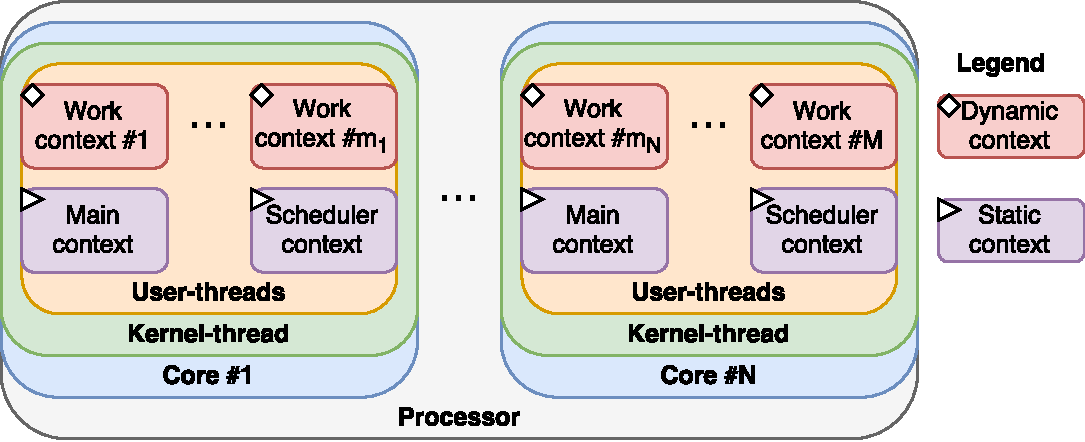
\includegraphics[width=0.9\linewidth]{fig/runtime_overview}
    \caption{Overview of the runtime system with $M$ work contexts, given $N$ online processor cores.}
    \label{fig:runtime_overview}
\end{figure}


%%%%%%%%%%%%%%%%%%%%%%%%%%%%%%%%%%%%%%%%
\subsection{Processes}
\label{subsec:process_implementation}


Processes are a vital part of \Proxc{}. As stated many times before, processes represents some kind of computation of the total program, which in code translates to running a function concurrently with the rest of the system. Constructing a process requires to supply a function pointer and its corresponding arguments. The process object constructs a context object out the function pointer and arguments, and stores an intrusive pointer to the context object as a data member. In other words, the process is no more than an opaque type to a context object. The programmer implicitly creates new contexts through processes, while the scheduler under the hood operates on the contexts. See \cref{lst:process_type} for reference.

\begin{lstfloat}
\begin{lstlisting}[caption={Minimal process type.}, label={lst:process_type}, style={CustomC++}, xleftmargin={2em}]
class Process {
private:
    using CtxPtr = boost::intrusive_ptr<proxc::Context>;
    CtxPtr ctx_ptr_{ nullptr };
public:
    template<typename Fn, typename... Args>
    Process(Fn && fn, Args &&... args);
};
\end{lstlisting}
\end{lstfloat}

The context objects represent the execution state of the computation. Each context object contains an execution context, which is the actual execution state of the computation. The execution context is implemented by the Boost Context library, which encapsulates context switching and manages the associated contexts stack. Note that a context object refers to the context type defined by the runtime system, and execution context refers to the Boost Context object which defines the actual processor state.

The context object does not implement much functionality, other than wrapping the execution context state with additional control structure data and intrusive data members. The functionality is implemented in the scheduler, which is explained in further detail in \cref{subsec:scheduler_implementation}.

Execution contexts can either create a context of the current running execution context, or takes a function pointer of the type \lstinline[style={CustomC++}]|void(void*)|. Transfer of control flow between execution contexts is done by calling another execution context with the overloaded \lstinline[style={CustomC++}]|void* operator()(void*)| method. Parameter passing is possible through void pointer casting. When transferring control to another execution context, an optional pointer can be passed. If this is the first transfer of control to the execution context, the parameter will be passed as the void pointer argument for the function. Else, the void pointer will be passed as the return value of the transfer of control operator.

\Cref{lst:transfer_control_execution_contexts} gives an example of how execution contexts work. An execution context of the current running context is made, as well as an execution context of a lambda function. The output of the code snippet will print \texttt{main} and \texttt{work} in that order. Refer to the Boost Context documentation for more thorough explanation of the execution context implementation \citep{kowalke2017boost}.

\begin{lstfloat}
\begin{lstlisting}[caption={Transfer of control between execution contexts.}, label={lst:transfer_control_execution_contexts}, style={CustomC++}, xleftmargin={2em}]
using ex_ctx = boost::context::execution_context;
ex_ctx main_ctx{ex_ctx::current()};
ex_ctx work_ctx{[&main_ctx](void* vp){
    std::string* msg = static_cast<std::string*>(vp);
    std::cout << *msg << std::endl;
    // prints `main`
    std::string work_msg{"work"};
    // transfer of control to main_ctx
    main_ctx(static_cast<void*>(&work_msg));
    // never returns
}};
std::string main_msg{"main"};
// transfer of control to work_ctx
void* vp = work_ctx(static_cast<void*>(&main_msg));
std::string* msg = static_cast<std::string*>(vp);
std::cout << *msg << std::endl;
// prints `work`
\end{lstlisting}
\end{lstfloat}

When creating a context object, an enclosing entry function of the type \lstinline[style={CustomC++}]|void(void*)| is created, which calls the received function with its arguments. This entry function, called trampoline, handles the void pointer argument from the execution context, calls the process function, and calls the terminate procedure when the process function returns. This way, all terminating processes can be gracefully resolved by the trampoline invisible to the programmer. Entry functions are created with generic lambdas, allowing to create generic entry function calling over any type of function pointer and arguments. This is explained in further detail in \cref{subsec:scheduler_implementation}.

The context object contains the type of the context, the execution context, the entry function for the particular process, and a pointer to the parent scheduler. Each process also has its own spinlock, used when synchronizing on certain inter\hyp{}process synchronization. Additionally, control data used by the scheduler is stored in the context object, such as intrusive hooks and time points for timed suspension. See \cref{lst:context_type} for a stripped down version of the context class definition.

\begin{lstfloat}
\begin{lstlisting}[caption={Minimal context type.}, label={lst:context_type}, style={CustomC++}, xleftmargin={2em}]
class Context {
private:
    using ExCtxT = boost::context::execution_context;
    using EntryFn = delegate<void(void*)>;
    using TimePointT = std::chrono::steady_clock::time_point;
    ExCtxT ex_ctx_;
    EntryFn entry_fn_{ nullptr };
    proxc::Scheduler * scheduler_ptr_{ nullptr };
public:
    TimePointT time_point_{ TimePointT::max() };
    proxc::Alt * alt_{ nullptr };
    proxc::Spinlock splk_;
    /* impl defined */ wait_queue_{};
    /* intrusive data members */
};
\end{lstlisting}
\end{lstfloat}

FIXME wait queue.


%%%%%%%%%%%%%%%%%%%%%%%%%%%%%%%%%%%%%%%%
\subsection{Scheduler}
\label{subsec:scheduler_implementation}


The scheduler is the corner piece of runtime system. It has the sole responsibility of managing the different processes, including creating, scheduling, and synchronizing processes. The scheduler runs as its own context, invisible to the programmer.

When the scheduler is initialized by the runtime initialization procedure, the scheduler context enters the scheduler event loop. The scheduler event loop is where the scheduler context resides during the lifetime of the entire program.

A scheduler is implemented as a class object, consisting of context queues and process management logic. See \cref{lst:scheduler_type} for reference.

\begin{lstfloat}
\begin{lstlisting}[caption={Minimal scheduler type.}, label={lst:scheduler_type}, style={CustomC++}, xleftmargin={2em}]
class Scheduler {
private:
    struct Initializer;
    bool exit_{ false };
    proxc::Context* running_ptr_{ nullptr };
    proxc::Spinlock splk_;
    /* impl defined */ policy_;
    /* impl defined */ work_queue_{};
    /* impl defined */ sleep_queue_{};
    /* impl defined */ terminated_queue_{};
    /* impl defined */ remote_queue_{};
public:
    static proxc::Scheduler* self();
    static proxc::Context* running();
};
\end{lstlisting}
\end{lstfloat}


%%%%%%%%%%%%%%%%%%%%%%%%%%%%%%%%%%%%%%%%
\subsubsection{Scheduler Initialization}


The scheduler has two static methods: \lstinline[style={CustomC++}]|self()| and \lstinline[style={CustomC++}]|running()|. The \lstinline[style={CustomC++}]|self()| method returns a pointer to the scheduler object which is the parent scheduler for the current running kernel\hyp{}thread, and can be called from any context. The \lstinline[style={CustomC++}]|running()| method returns a pointer to the context object currently running on the kernel\hyp{}thread, and can be called from any context.

The \lstinline[style={CustomC++}]|self()| method is the starting point of the runtime system, for which the first call to will trigger the initialization procedure. The method contains a static thread local variable of the scheduler initializer object, which is a Schwarz counter. A Schwarz counter, also known as a nifty counter, is a C++ idiom for ensuring a non\hyp{}local static object is initialized before its first use and destroyed only after last use of the object, where the non\hyp{}local static object in this case is the scheduler object. 

The first call to the scheduler initializer constructor on each kernel\hyp{}thread will initialize the scheduler object for the corresponding kernel\hyp{}thread, and simultaneously set its static thread local pointer member to the scheduler object. This static thread local pointer is the pointer which is returned by \lstinline[style={CustomC++}]|self()| method. Additionally, the \lstinline[style={CustomC++}]|running()| method returns the \lstinline[style={CustomC++}]|running_ptr_| member from the returned scheduler object, which is retrieved by the \lstinline[style={CustomC++}]|self()| method.

\begin{lstfloat}
\begin{lstlisting}[caption={Static scheduler methods.}, label={lst:static_scheduler_methods}, style={CustomC++}, xleftmargin={2em}]
// Schwarz counter
struct Scheduler::Initializer {
    thread_local static Scheduler* self_{ nullptr };
    thread_local static std::size_t counter_{ 0 };
    Initializer() {
        if (counter_++ == 0) { 
            /* initialize scheduler */ 
            /* member self_ is set */
        }
    }
    ~Initializer() {
        if (--counter_ == 0) { /* destroy scheduler */ }
    }
};
Scheduler* Scheduler::self() {
    thread_local static Initializer init;
    return Initializer::self_;
}
Context* Scheduler::running() {
    return Scheduler::self()->running_;
}
\end{lstlisting}
\end{lstfloat}


%%%%%%%%%%%%%%%%%%%%%%%%%%%%%%%%%%%%%%%%
\subsubsection{Process Queues}


From \cref{lst:scheduler_type} a total of five queues are used by the scheduler for process management: \textit{ready}, \textit{work}, \textit{sleep}, \textit{terminated} and \textit{remote} queue. 

The ready queue is called a scheduling policy, or just policy for short. The scheduling policy is an abstraction for the scheduler, for which ready processes are enqueued to and ready processes to resume are dequeued from. The scheduling policy is responsible to store the ready processes, and how and in which order the processes are enqueued and dequeued is up to the implementation of the scheduling policy. The default policy, which is hard coded as of now, is the work stealing policy. However, any type of scheduling policy could be implemented, such as round robin. Following the algorithm described in \cref{subsec:work_stealing_algorithm}, the queue is implemented as a combination of a double\hyp{}ended queue, deque for short, and a doubly linked list. The deque is used for dynamic processes and the doubly linked list is used for static processes. This is to avoid static processes from being stolen by other schedulers. The deque has two distinct ends called \textit{top} and \textit{bottom}. Enqueueing and dequeueing a dynamic process to the dequeue pushes and pops the process from the bottom end, respectively. The doubly linked list acts as a FIFO queue. The work stealing commences when both the deque and the doubly linked list are empty. A deque from another scheduler is chosen at random, and a process is tried to be stolen from the top end. Pointers to all deques from all schedulers are stored in a static list. Note that work stealing is happening unbeknownst to the scheduler, as the scheduler only enqueues and dequeues processes to the scheduler policy. 

The work queue, which holds all processes the scheduler is the parent of, is implemented as an intrusive doubly linked list. The sleep queue, which holds all processes suspended until a time point, is implemented as an intrusive multiset\footnote{A multiset is an associative container that contains a set of objects, which allows multiple keys with the same values.}. The terminated queue, which holds all process which has terminated and can be destroyed, is implemented as an intrusive doubly linked list. Both work, sleep and terminated queues are only manipulated by a single scheduler and are therefore not thread\hyp{}safe, i.e. no other schedulers can access these queues safely.

The remote queue is a concurrent MPSC queue, where the managing scheduler is the consumer while any other schedulers are the producers. Whenever a scheduler reschedules a process and it is now the parent scheduler, the context is placed in the remote queue to the parent scheduler. The parent scheduler transitions proecsses in the remote queue and enqueues them in the scheduling polict. In essence, the remote queue is used to signal schedulers when their processes are to be rescheduled, since remote schedulers cannot safely access the scheduling policy.


%%%%%%%%%%%%%%%%%%%%%%%%%%%%%%%%%%%%%%%%
\subsubsection{Process States and Transitions}


The scheduler imposes a set of states for a process and how a process transitions between these states. An overview of the finite state machine of the states and transitions are shown in \cref{fig:context_states}. The different different process states implies the following:

\begin{itemize}[topsep=0em,itemsep=-1em,partopsep=0.5em,parsep=1em]
    \item \textbf{Ready} -- a newly created process always starts in the ready state. A ready process is enqueued to a ready queue and is ready to be resumed by the parent scheduler.
    \item \textbf{Running} -- a process is currently executing on a kernel\hyp{}thread.
    \item \textbf{Ended} -- a process has terminated and is enlisted in the terminated queue. An ended process is can be destroyed by the parent scheduler.
    \item \textbf{Suspend} -- a process is waiting indefinitely. An another process might reschedule the suspended process.
    \item \textbf{Sleep} -- a process is waiting until a given time point. A sleeping process is enlisted in the sleep queue and is rescheduled by the parent scheduler when the time point has expired or is rescheduled by an another process.
    \item \textbf{Join} -- a process is waiting for an another process to terminate. The joining process is enlisted in the wait queue of the process to terminate, and will be rescheduled when the process terminates.
    \item \textbf{Remote} -- a process is rescheduled by an another process which does not have the same parent scheduler. A remote ready process is enlisted in the remote queue.
\end{itemize}

Some observations can be made by the transition diagram in \cref{fig:context_states}. A ready process can only transition to running. Only a running process can terminate. A transition to and from running is the same as a context switch between two processes. Remote state can be seen as an intermediate ready state. When a running process transitions from running to one of the states suspend, sleep or join, the next transition must be ready state. A transition between the three states suspend, sleep or join cannot occur.

\begin{figure}[h!]
    \centering
    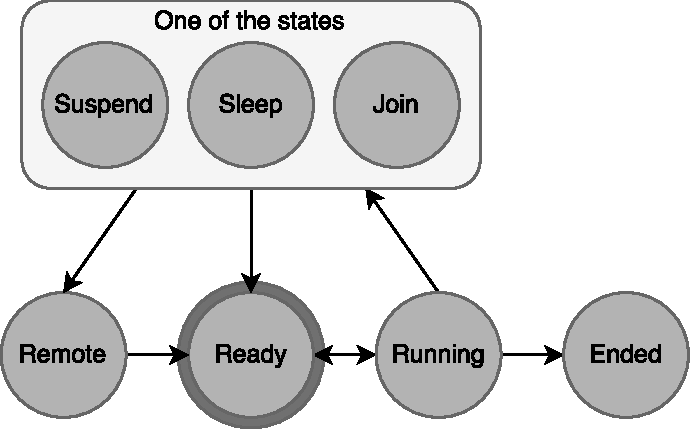
\includegraphics[width=0.7\linewidth]{fig/context_states}
    \caption{Finite state machine of states and transitions for a process.}
    \label{fig:context_states}
\end{figure}


%%%%%%%%%%%%%%%%%%%%%%%%%%%%%%%%%%%%%%%%
\subsubsection{Scheduler Functionality}


The scheduler implements a set of methods for manipulating processes, such as process management and inter\hyp{}process synchronization. It is important the scheduler implements the necessary functionality, as this forms the basis of what library features can be implemented. The follow functionality is available for a process:

\begin{itemize}[topsep=0em,itemsep=-1em,partopsep=0.5em,parsep=1em]
    \item \textbf{Process attaching and detaching} -- allows a process to be attached and detached to a scheduler, i.e. setting and removing a parent scheduler to a process.
    \item \textbf{Process rescheduling} -- allows a process to reschedule other processes.
    \item \textbf{Process suspension} -- allows a process to suspend execution, either indefinitely, for an another process, or until a given time point. 
    \item \textbf{Inter\hyp{}process synchronization} -- allows a process to synchronize on other processes, meaning the process waits for the other process to terminate.
    \item \textbf{Context switch operations} -- allows a process to perform certain operations immediately after context switch.
\end{itemize}

To further elaborate on the points above, attaching and detaching a process is necessary when work stealing. As all schedulers has a set of process of which it is responsible for, attaching a process is to register this responsibility. Detaching would unregister this responsibility. When a process migrates between two schedulers, the process must detach of its previous parent scheduler and attach to its new parent scheduler. 

a process rescheduling an another process requires checking whether they have the same parent scheduler or not. With the same parent scheduler, the process is enlisted directly to the ready queue. If different parent schedulers, the process is first enlisted to the remote queue, then enlisted to the ready queue when the parent schedulers transitions the process. If a rescheduled process was currently suspended with a timeout, the process is also removed from the sleep queue when enlisted to the ready queue.

Process suspension falls into two categories: waiting until some time point, or wait indefinitely. A process waiting until some time point enlists the process to the sleep queue. However, it is possible for other processes to reschedule the waiting process before the timeout occurs. A process waiting indefinitely may only be rescheduled by other processes.

Inter\hyp{}process synchronization, also called joining, allows for processes to wait for other processes to terminate. Each process has its corresponding spinlock, which is used to give mutual exclusion to the process termination flag. When a process terminates, the lock is acquired and the wait queue is checked. All processes enlisted to the wait queue is rescheduled and lastly the lock is released. On the other side when a process joining on an another process, the lock is first acquired and the termination flag is checked. If the termination flag is not set, the process enlists itself on the wait queue of the joining process, and the process suspends itself with releasing the lock. If the termination flag is set, the operation returns immediately. Note that it is safe for processes to access the wait queue as its guarded with mutual exclusion.

Context switch operations allows for processes to perform an action after the context switch has occurred. This is necessary when a process can only perform said action after itself has yielded execution. Currently, two operations requires a context switch operation: releasing a lock and rescheduling a process. Releasing a lock after a context switch is necessary when a process releasing a lock could result in the given process being rescheduled by an another process. An example of this is inter\hyp{}process synchronization. Rescheduling a process after a context switch is necessary when a process want to reschedule itself, such as processor yielding.


\FloatBarrier
%%%%%%%%%%%%%%%%%%%%%%%%%%%%%%%%%%%%%%%%
\subsubsection{Scheduler Event Loop}


The scheduler event loop is the where the entirety of the scheduler process is executing. The event loop consists of the following: check exit condition, process cleanup, process transitions, and process scheduling. See \cref{lst:scheduler_event_loop} for pseudo code reference.

What is important to note is that whenever the scheduler context switches to an another process, the scheduler process is enqueued to the ready queue before context switching. This ensures the scheduler is always available to context switch back to when running as a process. 

\begin{lstfloat}
\begin{lstlisting}[caption={Scheduler event loop pseudo code.}, label={lst:scheduler_event_loop}, style={CustomC}, xleftmargin={2em}]
while ( true ) {
    if (exit_condition()) {
        break;
    }
    // cleanup terminated contexts
    cleanup_terminated();
    // transition contexts to ready
    transition_remote(); // remote -> ready
    wakeup_sleep();      // sleep  -> ready
    // schedule ready context if any. Else, wait
    context = scheduling_policy.dequeue();
    if (context != nullptr) {
        // scheduler must always be available
        scheduling_policy.enqueue( scheduler_context );
        // context switch to ready process
        context.resume();
        // scheduler is now running
    } else {
        // sleep until first timeout or idle wakeup
        scheduling_policy.suspend_until( next_wakeup() );
    }
}
// scheduler is exiting, cleanup scheduler
scheduler_cleanup();
// lastly, context switch to main
main_context.resume();
// never returns
\end{lstlisting}
\end{lstfloat}

\FloatBarrier
%%%%%%%%%%%%%%%%%%%%%%%%%%%%%%%%%%%%%%%%%%%%%%%%%%%%%%%%%%%%%%%%%%%%%%%%%%%%%%%%
\section{Library Feature Implementations}

Library features provides the framework for the library for which are visible for the programmer. All features use the runtime system to implement its functionality, and this section explains this in further detail.


%%%%%%%%%%%%%%%%%%%%%%%%%%%%%%%%%%%%%%%%
\subsection{Timers}


The three types of timers described in \cref{subsec:timers_desgin} are represented through a common abstract class interface, shown in \cref{lst:timer_class_interface}. Instances of an egg or repeat timer converts the specified time duration to a time point, while the date timer already specifies a time point. This time point is stored in the base interface class. All timers support duration and time points from the standard library \lstinline[style={CustomC++}]|std::chrono|.

\begin{lstfloat}
\begin{lstlisting}[caption={Timer class interface.}, label={lst:timer_class_interface}, style={CustomC++}, xleftmargin={2em}]
class timer::Interface {
protected:
    using TimePointT = /* implementation defined */;
    TimePointT time_point_;
public:
    virtual void reset() = 0;
    virtual bool expired() = 0;
    bool operator<( Interface const & other ) const 
    { return time_point_ < other.time_point_; }
    TimePointT const & get() const { return time_point_; }
};
\end{lstlisting}
\end{lstfloat}

When a timer is supplied for a timed operation, the reset method is called. For the egg timer, a reset results in calculating new time point. For the repeat timer, the next periodic time point is calculated if expired, else the time point remains the same.

Multiple timers can be supplied for some operations, such as alting. Since timers have a static time point after a reset, the closest time point is chosen for timeout when there are multiple timers.

An explicit process suspension with a given timer is simply enlisting the process to the scheduler sleep queue with the corresponding time point. When the time point is reached, the scheduler will transition the process from the sleep queue to the ready queue. The time points are checked by the scheduler process in the scheduler event loop with the \texttt{Scheduler::wakeup\_sleep()} method. Suspending a process with a timer will immediately return if the time point is already reached.

A timed operation differs slightly from a timed suspension. Whenever the process waits for some event during the operation, the process is enlisted in the sleep queue. Now, one of two things may happen: either the process is rescheduled by some other process, or the operation times out and is rescheduled by the scheduler. If the process was rescheduled by some other process, the scheduler removes the process from the sleep queue and is enqueued in the ready queue. If the time point expires, the scheduler transitions the process from the sleep queue to the ready queue just as a timed suspension. Either way, the process is removed from the sleep queue and enqueued in the ready queue.

Note that if the process is rescheduled by some other process which does not share the same parent scheduler, the process is enlisted in the remote queue first, but is not removed from the sleep queue. It is not until the scheduler transitions the process from remote to ready during the \texttt{Scheduler::transition\_remote()} procedure the process is removed from the sleep queue.


%%%%%%%%%%%%%%%%%%%%%%%%%%%%%%%%%%%%%%%%
\subsection{Parallel Statement}


The parallel statement has two obvious phases: the \textit{fork} and \textit{join phase}. 

During the fork phase, each process to be executed in parallel is spawned by the parent process, one by one. The parent process is in this context the process calling the parallel statement. Spawning involves creating the process, attaching the process to the current scheduler, and launching the process. Launching the process simply enqueues the process to the ready queue of the current scheduler. When all parallel process has been spawned, the parent process enters the join phase.

The join phase consists of the parent process joining all parallel processes, one by one. Joining a process involves waiting until the process has terminated. One of two things happen when joining: either the process has not terminated and is still executing, or it has terminated. If the process has terminated, the parent process continues the join phase. If not, the parent process waits. When the process terminates, it will wake up the parent process.

Pseudo code for the parallel implementation is presented in \cref{lst:parallel_statement_pseudo_code}.

\begin{lstfloat}
\begin{lstlisting}[caption={Parallel statement pseudo code.}, label={lst:parallel_statement_pseudo_code}, style={CustomC++}, xleftmargin={2em}]
/* fork phase */
for_each process in parallel_processes {
    process.fork();
}
/* join phase */
for_each process in parallel_processes {
    process.join();
}
\end{lstlisting}
\end{lstfloat}

The parallel statement is quite simplistic, as it only enqueues new processes to the current scheduler and waits for their termination. Much of the simplicity comes from the lack of a \textit{sequential} statement, simplifying the design significantly. 


%%%%%%%%%%%%%%%%%%%%%%%%%%%%%%%%%%%%%%%%
\subsection{Channels}


Following the design in \cref{subsec:channel_design}, channels exist in one flavour: synchronous and unbuffered, unidirectional, one\hyp{}to\hyp{}one, and type safe. 

Channel objects are of the type \lstinline[style={CustomC++}]|Chan<T>|, which are composed of the two channel end objects \lstinline[style={CustomC++}]|Chan<T>::Tx| and \lstinline[style={CustomC++}]|Chan<T>::Rx|. \lstinline[style={CustomC++}]|Tx| and \lstinline[style={CustomC++}]|Rx| can send and receive on a channel, respectively. Creating a channel object allocates the two channel ends with the \lstinline[style={CustomC++}]|channel::create<T>()| method. The two channel ends are accessible via channel methods. The channel method \lstinline[style={CustomC++}]|Chan<T>::ref_tx/rx()| returns a reference to either channel end, while the method \lstinline[style={CustomC++}]|Chan<T>::move_tx/rx()| returns a moved channel end object. See \cref{lst:channel_object_type} for reference.

\begin{lstfloat}
\begin{lstlisting}[caption={Channel object type.}, label={lst:channel_object_type}, style={CustomC++}, xleftmargin={2em}]
template<typename T>
struct Chan : public std::tuple<Tx<T>,Rx<T>> {
    using Tx = Tx<T>;
    using Rx = Rx<T>;
    using TplT = std::tuple<Tx<T>,Rx<T>>;
    Chan() : TplT{ channel::create() } {}
    Tx & ref_tx();  Rx & ref_rf();
    Tx   move_tx(); Rx   move_rx();
};
\end{lstlisting}
\end{lstfloat}

Two channel containers are also supplied: \lstinline[style={CustomC++}]|ChanArr<T,N>| for static allocation on the stack, and \lstinline[style={CustomC++}]|ChanVec<T>| for dynamic allocation on the heap. The underlying container of \lstinline[style={CustomC++}]|ChanArr<T,N>| is a \lstinline[style={CustomC++}]|std::array<T,N>|, and the underlying cotnainer of \lstinline[style={CustomC++}]|ChanVec<T>| is a \lstinline[style={CustomC++}]|std::vector<T>|. All related methods and types associated with the underlying container is accessible with the corresponding channel container. This means channel containers support indexing with brackets, e.g. \lstinline[style={CustomC++}]|[i]|. See \cref{lst:channel_container_types} for channel container type definitions.

\begin{lstfloat}
\begin{lstlisting}[caption={Channel container types.}, label={lst:channel_container_types}, style={CustomC++}, xleftmargin={2em}]
template<typename T, std::size_t N>
struct ChanArr : public std::array<T,N> {
    using ArrT = std::array<T,N>;
    using ArrT::ArrT;
    ChanArr() : ArrT() {}
};
template<typename T>
struct ChanVec : public std::vector<T> {
    using VecT = std::vector<T>;
    using VecT::VecT;
    ChanVec(std::size_t n) : VecT(n) {}
};
\end{lstlisting}
\end{lstfloat}

Both channel containers has the methods \lstinline[style={CustomC++}]|collect_tx/rx()|, which returns a container of all corresponding channel ends in the container. The returned container type is the same as the underlying channel container.

Channel operations on a channel end, alting or not, can be timed with a timer. Both sending and receiving channel ends can be used in alting, compared to occam and XC which only permits receiving channel ends.

Channels can be closed. When a channel is closed, no more channel operations can be completed on the given channel. Closing a channel cannot be undone. A channel closes when either one of the channel ends goes out of scope, or one the channel ends explicitly closes the channel.

Channel ends are movable but non\hyp{}copyable, meaning channel ends must explicitly pass ownership between scopes. As each process in itself is an independent running scope, channel ends being non\hyp{}copyable ensures only one process holds and owns a channel end at any given time. If a process where to pass a channel end to another process, the ownership of the given channel end must be moved.

Channel ends are no more than class object holding a shared pointer to the underlying channel implementation. The channel implementation is of type \lstinline[style={CustomC++}]|ChannelImpl<T>|, containing the entire channel functionality. Channel ends are therefore no more than wrapping types restricting the access to the channel implementation. Whenever a channel is to be allocated, a channel implementation object is dynamically allocated with the shared pointer \lstinline[style={CustomC++}]|std::shared_ptr<T>|, and both channel ends are constructed with the shared pointer of the channel implementation.

The channel implementation follows the algorithm presented in \cref{subsec:channel_end_algorithm}. Some important details to note is that all channel operations, such as closing, send, receive, etc. are enclosed with a spinlock that belongs to the channel implementation object. This effectively serializes all access to the channel implementation. However, some parts of the channel end algorithm requires the participant to wait. The lock is therefore released after the process is suspended, using a context switch operation. If the lock were to be released before suspending, the opposite channel end could theoretically complete the channel operation and reschedule the current channel end before it suspended.

The alting channel end implementation is slightly more complicated than the non\hyp{}alting implementation, as it has a alt\hyp{}to\hyp{}alt synchronization procedure before trying the acquire the channel implementation lock.


%%%%%%%%%%%%%%%%%%%%%%%%%%%%%%%%%%%%%%%%
\subsection{Alting}


The alting procedure is implemented as a class object of type \lstinline[style={CustomC++}]|Alt|, which is allocated on the stack. The channel alternative is composed into two different channel alternative objects, each for the sending and receiving case. Both alternative objects inherit from a common abstract class interface. The timer and skip alternatives are both allocated as a data member in the alting object. 

After creating an alting object, alternatives can be created by chaining function calls to the alting object. The four functions \texttt{send}, \texttt{recv}, \texttt{timeout} and \texttt{skip} creates a channel send, channel receive, timeout and skip alternative, respectively. The channel alternative functions has a corresponding replicator function for creating dynamic number of channel alternatives over a dynamic number of channel ends These are called \texttt{send\_for} and \texttt{recv\_for}. All alternative creating functions also has an corresponding guarded function, which is the function name with \texttt{\_if} appended, e.g. \texttt{send\_if}. Lastly, the function call \texttt{select} performs the alting procedure and consumes the alting object in the process. The \texttt{select} function call is always last. See \cref{lst:code_example_alting} for a code example.

\begin{lstfloat}
\begin{lstlisting}[caption={Code example of alting.}, label={lst:code_example_alting}, style={CustomC++}, xleftmargin={2em}]]
Alt()                           // creates alting object
    .send(tx, item)             // w/o guard, w/o closure
    .recv_if(cond1, rx)         // w   guard, w/o closure
    .timeout(timer, [](){})     // w/o guard, w   closure
    .skip_if(cond2, &some_func) // w   guard, w   closure
    /* more alternatives can be inserted here */
    .select();                  // selects an alternative
\end{lstlisting}
\end{lstfloat}

An important observation to make is that all alternative functions simply generate and store alternatives in the alting object. However, some additional care has to be taken into consideration. Multiple alternatives can be created on the same channel end. If this is the case, then the alting object chooses one at random for which is used during the alting procedure. If both ends of the same channel is detected as alternatives, then all alternatives for that channel are discarded.

Timeout alternatives are stored as a single entry in the alting object. Whenever a timeout alternative is created, the timeout period is checked against the current timeout period, initialized to maximum value. If the timeout period is lower than the current one, the new timeout alternative is swapped in place.

Skip alternatives are stored as a single entry in the alting object. Compared to the timeout alternative, only the first skip alternative is stored. All subsequent skip alternatives are discarded.

The alting procedure follows the algorithm presented in \cref{subsec:alting_algorithm}. A spinlock is used for mutual exclusion during the alting procedure to enforce active and passive selection. An atomic flag and a pointer is used to set the ``winner'' of the selection. \Cref{lst:active_alting,lst:passive_alting} shows an illustration of the active and passive alting.

During the checking phase, the alting object holds the lock. If the alting procedure actively selects an alternative, the atomic flag is set and the pointer is set accordingly. Only after alting procedure continues to the waiting or completing phase is the lock released. Any alternative that becomes ready during the checking phase and tries to select passively must acquire the alting lock first. This allows the alting procedure to enforce all alternatives trying to passively select to wait until the waiting or completing phase. 

If the alting procedure enters the waiting phase, the alting procedure suspends itself and the lock is released. Note that the lock is released after the suspension, using context switch operation.  The first alternative to acquire the lock and set the atomic flag is allowed to set the winner pointer. This alternative also reschedules the alting procedure.

\begin{lstfloat}
\begin{lstlisting}[caption={Code example of alting.}, label={lst:active_alting}, style={CustomC++}, xleftmargin={2em}]]
lock = spinlock.aquire();
ready_selected = checking_phase();
winner = if ! ready_selected {
    if skip { skip_alternative }
    else {
        // atomically suspend and release lock
        timeout = scheduler.alt_wait( lock );
        if timeout { timeout_alternative }
        else       { channel_alternative }
    }
} else { ready_alternative };
completing_phase(winner);
\end{lstlisting}
\end{lstfloat}

\begin{lstfloat}
\begin{lstlisting}[caption={Code example of alting.}, label={lst:passive_alting}, style={CustomC++}, xleftmargin={2em}]
lock = spinlock.aquire();
if ! alt.atomic_flag.test_and_set() { return false; }
alt.winner = channel_alternative;
scheduler.reschedule(alt.context);
return true;
\end{lstlisting}
\end{lstfloat}

The alting procedure uses a uniform random distribution to randomly choose an alternative if multiple alternatives are ready during the active phase. Using a uniform random distribution makes the alting procedure fair and non\hyp{}deterministic. Whether an alting procedure prefers determinism over fairness or not is not up for this thesis to discuss, and for all practical reasons the alting procedure favors fairness over determinism.


% !TEX encoding = UTF-8 Unicode
%!TEX root = main.tex
% !TEX spellcheck = en-US
%%=========================================


%%%%%%%%%%%%%%%%%%%%%%%%%%%%%%%%%%%%%%%%%%%%%%%%%%%%%%%%%%%%%%%%%%%%%%%%%%%%%%%%
\chapter{Examples of Usage}
\label{ch:examples_usage}

This chapter introduces how \Proxc{} is used in \Cpp{} programs. Only the basics of \Proxc{} is presented, introducing all necessary features for understanding the library. First of all, \Proxc{} must be installed on the work environment. \Proxc{} is available for free as in beer on GitHub \citep{pettersen2017proxcgithub}. Following the install guide on the readme should be sufficient. For more advanced examples, check out the examples in the \texttt{examples/} folder on the GitHub project.

All library related types and methods reside in the \lstinline[style={CustomC++}]|proxc| namespace, which will be omitted in all code examples. It is given the header file \lstinline[style={CustomC++}]|#include <proxc.hpp>| is included in all code examples shown in this chapter, as well as in all \Cpp{} files programming with \Proxc. The linker flag \lstinline[style={CustomC++}]|-lproxc| must also be passed during compilation.

Programs using \Proxc{} does not need to initialize or cleanup the library. This is done automatically by the library. The first call to the library which invokes the runtime system will initialize the library, and the cleanup procedure is invoked when the program exits. No cleanup will be invoked unless the library has been initialized. 


%%%%%%%%%%%%%%%%%%%%%%%%%%%%%%%%%%%%%%%%
\section{Processes}


At the core of \Proxc{} are lightweight processes. These processes is a separate scope of execution which can run concurrently with the rest of the program. In code, these processes are represented by a function and its corresponding arguments. The main function of any \Cpp{} program is also implicitly a process. This function must have a return type of \lstinline[style={CustomC++}]|void|, but can have any type and number of arguments. \Cref{lst:code_example_process_func} shows different function prototypes where some qualify running as a process and some do not.

\begin{lstfloat}
\begin{lstlisting}[caption={Different function prototypes which do and do not qualify as a process.}, label={lst:code_example_process_func}, style={CustomC++}, xleftmargin={2em}]
void good_func1();                // ok
void good_func2(std::string msg); // also ok
int         bad_func1();      // not ok, return type not void
std::string bad_func2(int y); // also not ok
\end{lstlisting}
\end{lstfloat}

Processes are stored as process objects of the type \lstinline[style={CustomC++}]|Process|. These process objects can be created and stored freely in any container. A process object can be created explicitly with the object constructor, which takes a function pointer and its corresponding arguments. Or, a process object can be created implicitly with the library method \lstinline[style={CustomC++}]|proc|. \Cref{lst:process_creation} illustrates the difference.

\begin{lstfloat}[h!]
\begin{lstlisting}[caption={Process creation.}, label={lst:process_creation}, style={CustomC++}, xleftmargin={2em}]
Process my_process{&my_func, arg1, arg2};
auto other_process = proc(&other_func, other_arg);
\end{lstlisting}
\end{lstfloat}

Process creation also has perfect forwarding of arguments, meaning any type of arguments being expensive to copy or being non\hyp{}copyable can correctly be moved into processes.

A dynamic number of processes can also be created, which requires to either explicitly allocate each process before hand in any container or to generate them on the fly. The library method \lstinline[style={CustomC++}]|proc_for| takes either a pair of input iterators to any container of processes, or a pair of integers which defines the integer range $[\text{start},\text{end}\rangle$ and a function pointer which takes an integer as an argument. The method returns a process which runs the dynamic numbers of processes in parallel. See \cref{lst:dynamic_number_process_creation} for reference. Calling the \lstinline[style={CustomC++}]|proc_for| method only creates the parallel process, and does not run them.

\begin{lstfloat}[h!]
\begin{lstlisting}[caption={Creating a dynamic number of processes.}, label={lst:dynamic_number_process_creation}, style={CustomC++}, xleftmargin={2em}]
std::vector<Process> procs;
for (int i = 0; i < N; ++i) 
    procs.emplace_back(&some_func, some_data[i]);
auto total_procs = proc_for(procs.begin(), procs.end());
// or
auto total_procs = proc_for(0, N,
    [&some_data](int i){ some_func(some_data[i]); });
\end{lstlisting}
\end{lstfloat}

Creating a process is not useful if it cannot be executed in parallel with the rest of the system. The library function \lstinline[style={CustomC++}]|parallel| takes one\hyp{}or\hyp{}more processes and runs them in parallel, following the fork\hyp{}join model. The calling process will suspend until all parallel processes has terminated. See \cref{lst:example_parallel_statement} for reference.

\begin{lstfloat}
\begin{lstlisting}[caption={Example of the parallel statement.}, label={lst:example_parallel_statement}, style={CustomC++}, xleftmargin={2em}]
std::vector<Process> procs;
// ...
parallel(
    proc(&my_func, 42),
    proc([](){ /* lambda function */ }),
    proc_for(procs.begin(), procs.end()),
    proc_for(0, N, &calculate_func)
);
\end{lstlisting}
\end{lstfloat}

Process objects are non\hyp{}copyable but movable, meaning the ownership of process objects must be moved between scopes. A process object is of one time use. After a process has executed and terminated, the process object cannot be run again. The process object must be constructed once more to be executed again. 

In any process context, a set of operations are available for the current running process, accessible in the \lstinline[style={CustomC++}]|this_proc| namespace. The operations includes getting the current process id, yielding, and suspending for a given duration or until a time point. The suspension operations supports time types from the standard library \lstinline[style={CustomC++}]|std::chrono|. See \cref{lst:per_process_operations} for reference.

\begin{lstfloat}
\begin{lstlisting}[caption={Per process operations for the current executing process.}, label={lst:per_process_operations}, style={CustomC++}, xleftmargin={2em}]
auto id = this_proc::get_id();
this_proc::yield();
this_proc::delay_for(/* duration */);
this_proc::delay_until(/* time point */);
\end{lstlisting}
\end{lstfloat}


%%%%%%%%%%%%%%%%%%%%%%%%%%%%%%%%%%%%%%%%
\section{Timers}
\label{sec:timer_example}


Three types of timers are available in \Proxc{}: egg, repeat and date timers. Timers allow for soft real\hyp{}time requirements on certain operations. All timers have support for time period and duration declarations using the standard time library \lstinline[style={CustomC++}]|std::chrono|.

All timer objects reside in the \lstinline[style={CustomC++}]|timer| namespace. Timer objects are constructed with a supplied appropriate duration or time point, and are both copyable and movable. See \cref{lst:creating_timers} for reference. 

\begin{lstfloat}
\begin{lstlisting}[caption={Constructing different timers.}, label={lst:creating_timers}, style={CustomC++}, xleftmargin={2em}]
timer::Egg    egg{/* duration */};
timer::Repeat rep{/* duration */};
timer::Date   date{/* time point */};
\end{lstlisting}
\end{lstfloat}

Egg timers are used for relative timeout periods. Just as an egg timer in real life, the timer starts when the operation starts, and expires when the time period has passed. The egg timer can be reused after expiration, as the countdown is reset every time it is supplied for an operation. In a sense, the timer does not ``survive'' between multiple operations, as it resets.

Repeat timers are used for periodic timeout periods. Given a time duration, the repeat timer will expire every period equal to the time duration. When supplied with an operation, the repeat timer does not reset. Only when it expires does it reset, basically setting the next timeout point to the next period forward in time. Repeat timers do ``survive'' between multiple operations, as only when it expires does it reset. 

Date timers are used for absolute timeout periods. Given a time point, the date timer will expire when current time point has surpassed the given time point. The date timer does ``survive'' between multiple operations, however will always stay expired after timeout. 


%%%%%%%%%%%%%%%%%%%%%%%%%%%%%%%%%%%%%%%%
\section{Channels}


Processes uses message\hyp{}passing to communicate, which is realized through channels. The philosophy of CSP\hyp{}based concurrency is processes should not share memory directly, as this is a potent problem often leading to race conditions. Rather, the processes should share memory by communicating, i.e. message\hyp{}passing with channels.

Channels in \Proxc{} exist only in one flavour: synchronous and unbuffered, unidirectional, one\hyp{}to\hyp{}one and type safe. Channel objects are of the type \lstinline[style={CustomC++}]|Chan<T>|, and takes no additional arguments in its constructor. Channel objects are non\hyp{}copyble but movable.

A channel object is a named tuple, containing the two channel end objects \lstinline[style={CustomC++}]|Chan<T>::Tx| and \lstinline[style={CustomC++}]|Chan<T>::Rx|, The channel ends \lstinline[style={CustomC++}]|Tx| and \lstinline[style={CustomC++}]|Rx| can respectively send and receive on the channel. Channel end objects are also non\hyp{}copyable but movable.

Channel ends can be access directly from the channel object via the class methods \lstinline[style={CustomC++}]|ref_tx| and \lstinline[style={CustomC++}]|ref_rx|, which returns a reference to the channel end objects. Channel end objects can also be moved from the channel object with the class methods \lstinline[style={CustomC++}]|move_tx| and \lstinline[style={CustomC++}]|move_rx|. See \cref{lst:channel_creation} for reference.

\begin{lstfloat}
\begin{lstlisting}[caption={Channel creation and channel end access.}, label={lst:channel_creation}, style={CustomC++}, xleftmargin={2em}]
Chan<std::string> channel;
/* channel end access */
channel.ref_tx();  /* and */ channel.ref_rx();
/* channel end move */
channel.move_tx(); /* and */ channel.move_rx();
\end{lstlisting}
\end{lstfloat}

Given a channel of type \lstinline[style={CustomC++}]|Chan<T>|, the channel end objects \lstinline[style={CustomC++}]|Tx| and \lstinline[style={CustomC++}]|Rx| can send data of the type \lstinline[style={CustomC++}]|T| over the channel. Channel transmissions has perfect forwarding of data.

The channel end object \lstinline[style={CustomC++}]|Tx| can either send data with the class method \lstinline[style={CustomC++}]|send| or with the overloaded \lstinline[style={CustomC++}]|operator<<|. The class method returns the explicit result of the operation, while the overloaded operator only returns a boolean of whether the operation was a success or not. See \cref{lst:sending_channel_end} for reference.

\begin{lstfloat}
\begin{lstlisting}[caption={Sending on the Tx channel end object.}, label={lst:sending_channel_end}, style={CustomC++}, xleftmargin={2em}]
Chan<long> channel;
auto tx = channel.move_tx();
auto op_result = tx.send(some_data); 
/* or */
bool success = tx << some_data;
\end{lstlisting}
\end{lstfloat}

The channel end object \lstinline[style={CustomC++}]|Rx| can either receive data with the class method \lstinline[style={CustomC++}]|recv| or with the overloaded \lstinline[style={CustomC++}]|operator>>|. An important difference from the sending operations is the receive data must be preallocated before calling the receive methods. However, the return types resembles the return types of sending. See \cref{lst:receiving_channel_end} for reference.

\begin{lstfloat}
\begin{lstlisting}[caption={Receiving on the Rx channel end object.}, label={lst:receiving_channel_end}, style={CustomC++}, xleftmargin={2em}]
Chan<long> channel;
auto rx = channel.move_rx();
long some_data; // received data must be preallocated!
auto op_result = rx.recv(some_data); 
/* or */
bool success = tx >> some_data;
\end{lstlisting}
\end{lstfloat}

Both channel end objects overload \lstinline[style={CustomC++}]|operator()| for inline sending and receiving. However, inline channel operations does not return any indications whether the channel operation was a success or not. See \cref{lst:inline_channel_operations} for reference.

\begin{lstfloat}
\begin{lstlisting}[caption={Inline channel operations.}, label={lst:inline_channel_operations}, style={CustomC++}, xleftmargin={2em}]
Chan<T>::Tx tx; Chan<T>::Rx rx;
tx(data); // returns void
rx();     // returns T
\end{lstlisting}
\end{lstfloat}

A channel has a notion of being open or closed. A channel always starts as being open. When a channel is closed, no more channel transmission can be completed. A closed channel forever remains closed until destroyed. A channel becomes closed either by a channel end explicitly closing the channel with the class method \lstinline[style={CustomC++}]|close|, or a channel end object goes out of scope and is deallocated. A channel end can test whether the channel is closed or not with the class method \lstinline[style={CustomC++}]|is_closed|, which returns true for a closed channel and false otherwise.

The channel end object \lstinline[style={CustomC++}]|Rx| supports for range\hyp{}based for loops, retrieving data as long as the channel is open. When the channel becomes closed, the for loop automatically break. See \cref{lst:range_based_for_loops_channel} for reference.

\begin{lstfloat}
\begin{lstlisting}[caption={Range\hyp{}based for loops with the receving channel end.}, label={lst:range_based_for_loops_channel}, style={CustomC++}, xleftmargin={2em}]
Chan<T>::Rx rx;
for (auto data : Rx) {
    /* do some work */
}
/* here, channel is closed */
\end{lstlisting}
\end{lstfloat}

A receiving channel end can pipe its input into a sending channel end, meaning all data received on the receiving channel end is forwarded as the output on a sending channel end. The overloaded \lstinline[style={CustomC++}]|operator>>| is used to pipe data between a receiving and sending channel end, which returns a boolean indicating success or not. A successful piping is only when data is successfully received and sent. If either operations fail, the piping operation failed as well. See \cref{lst:piping_channel_end} for reference.


\begin{lstfloat}
\begin{lstlisting}[caption={Piping from a receiving to sending channel end object.}, label={lst:piping_channel_end}, style={CustomC++}, xleftmargin={2em}]
Chan<T>::Tx tx; Chan<T>::Rx rx;
while (rx >> tx) { /* piping is successful */ }
/* piping failed */
\end{lstlisting}
\end{lstfloat}

Lastly, a channel send or receive operation can be timed. A time duration or time point from the standard library \lstinline[style={CustomC++}]|std::chrono| can be supplied with a channel operation. The channel operation will try to complete within the specified time, and returns either if the operation completed or timed out. The return value of the timed operation specifies the reason for the channel operation to returned.


%%%%%%%%%%%%%%%%%%%%%%%%%%%%%%%%%%%%%%%%
\section{Alting}


If a process were to wait on multiple channel ends simultaneously, normal channel operations would not suffice. The alting construct however allows a process to simultaneously wait on multiple channel operations and complete one when one becomes ready. The channel operations, together with timeouts and skips, makes up what is called alting alternatives.

The four alternatives are as follows: channel send and receive takes an appropriate channel end and data, and performs the given channel operation. A timeout specifies a timer and wait until that timer has expired. A skip is always ready, much like the default keyword in a switch construct. 

The alting procedure allows a process to synchronously wait for multiple alternatives. The alting procedure block the calling process until one of the alternatives can complete, and completes that alternative. A corresponding closure, which can be anything callable, is then executed if present. When the alting procedure finishes, including the executed closure has returned, the process resumes.

An alting procedure consists of zero\hyp{}or\hyp{}more alternatives, where the alting procedure waits for these alternatives to become ``ready''. When one\hyp{}or\hyp{}more alternatives are ready, the alting procedure chooses one alternative and executes a corresponding closure. Alternatives can be guarded by a boolean condition, which enables or disables an alternative for the alting procedure depending on the condition.

An alting procedure starts with creating an alting object of the type \lstinline[style={CustomC++}]|Alt|. This alting object can create alternatives by function chaining multiple alternative methods, and lastly call a selection method which consumes the alting object and resolves the alting procedure. See \cref{lst:alting_procedure} for reference.

\begin{lstfloat}
\begin{lstlisting}[caption={Example of the alting construct.}, label={lst:alting_procedure}, style={CustomC++}, xleftmargin={2em}]
Alt()
    .send(tx, 42)
    .recv_if(cond1, rx)
    .timeout(timer, &timeout_func)
    .skip_if(cond2, [](){
        /* skip lambda */
    })
    .select();
\end{lstlisting}
\end{lstfloat}

The four alternative types channel send, channel receive, timeout and skip has the corresponding alternative methods \lstinline[style={CustomC++}]|send|, \lstinline[style={CustomC++}]|recv|, \lstinline[style={CustomC++}]|timeout| and \lstinline[style={CustomC++}]|skip|, respectively. 

Each alternative method can prepend a guard with a boolean condition by calling the altered alternative method, which has an appended \lstinline[style={CustomC++}]|_if| to the method name, e.g. \lstinline[style={CustomC++}]|send_if|. All alternative methods, both with and without a guard, can have an optional closure. See \cref{lst:alting_procedure} for reference.

A dynamic number of channel send and receive alternatives can be generated. The class methods \lstinline[style={CustomC++}]|send_for| and \lstinline[style={CustomC++}]|recv_for| takes a pair of iterators to any container with the appropriate channel end object, and generates a correposnding alternative for each channel end. The class methods can also be guarded, following the same naming scheme as the single alternative methods. 

The timer alternatives takes on of the three timer types presented in \cref{sec:timer_example}. 


% !TEX encoding = UTF-8 Unicode
%!TEX root = main.tex
% !TEX spellcheck = en-US
%%=========================================

%%%%%%%%%%%%%%%%%%%%%%%%%%%%%%%%%%%%%%%%%%%%%%%%%%%%%%%%%%%%%%%%%%%%%%%%%%%%%%%%
\chapter{Performance}
\label{ch:performance}


Benchmarking performance of a concurrency library is not intuitive. Some might even argue performance is not important, but rather the abstractions are correct. However, some metrics of parallel programs can be tested.

For this benchmark, a set of concurrent programs are tested with various degrees of parallelism. Metrics such as concurrent throughput, sequential speed, and load balancing are factors which can influence performance.

To have some appropriately comparable benchmarks, entries from \cref{sec:multicore_csp_existing} are included. occam and XC are however not included, as they require proprietary hardware to run on multicore architectures. C++CSP2 is also not included because of difficulties of implementing benchmark tests which did not result in spurious segmentation faults by the library during execution.

Additionally, singlecore versions of \Proxc{} and Go are included to observe the potential speedup in performance with multicore. \Proxc{} implements a singlecore runtime system with a round robin scheduling policy, while Go implements singlecore runtime system by setting the number of schedulers to one with \texttt{GOMAXPROCS}. C++CSP has no support for a singlecore runtime system, and therefore only the multicore version is included.

All code for the different benchmark tests can be found in \cref{ch:benchmark_code}.


%%%%%%%%%%%%%%%%%%%%%%%%%%%%%%%%%%%%%%%%%%%%%%%%%%%%%%%%%%%%%%%%%%%%%%%%%%%%%%%%
\section{Benchmark Setup}
\label{sec:benchmark_setup}


All benchmarks performed in this chapter are computed on the same machine; a desktop PC with an Intel\textsuperscript{\textregistered} Core\textsuperscript{\texttrademark} i7-4790 4GHz processor with 8 logical cores, 16GiB DDR3 RAM, running Ubuntu\textsuperscript{\textregistered} 16.04 xenial, x86\_64 Linux\textsuperscript{\textregistered} 4.4.0 as operating system.

Intel Core is a registered trademark of Intel Corporation, Linux is the registered trademark of Linus Torvaldsen in the U.S. and other countries, Ubuntu is a registered trademark of Canonical Ltd.


%%%%%%%%%%%%%%%%%%%%%%%%%%%%%%%%%%%%%%%%%%%%%%%%%%%%%%%%%%%%%%%%%%%%%%%%%%%%%%%%
\section{Benchmark Tests}
\label{sec:benchmark_tests}


Three type of benchmark tests are performed: \textit{extended commstime}, \textit{concurrent mandelbrot} and \textit{concurrent prime sieve}. These three tests have various degrees of sequential and parallel characteristics, aiming to highlight the concurrency adaptation capabilities, the concurrent throughput, and how well each entry scales with an increasing amount of parallel work load.


%%%%%%%%%%%%%%%%%%%%%%%%%%%%%%%%%%%%%%%%
\subsection{Extended Commstime}


The extended commstime test is a custom derivation of the original commstime test. The original commstime test \citep{roger2001commstime} is a pseudo\hyp{}standard benchmark for testing sequential channel communication between processes. Three processes called \textit{prefix}, \textit{delta} and \textit{successor} creates a channel cycle, sending an integer in loops. Each loop increments the integer. A fourth process, called \textit{consumer}, receives the integer on each loop cycle. The consumer receives an integer a number of times and calculates the average time to receive the integer. The commstime test mostly gives a metric for the overhead regarding channel communication.

Channel communication overhead is not that interesting of a metric with dynamic multithreading. Commstime is however a good metric for a programs adaptability of sequential programs, as all processes create an sequential dependency. I therefore propose the \textit{extended commstime} test. Instead of three processes in a channel communication cycle, $N$ processes are created in a chain of channel communications, creating a variable sized cycle.

The extended commstime varies the chain length from $N=1$ to $1000$. For each chain length value of $N$, the time to receive $100$ integers divided by the chain length is averaged over $50$ runs. 

The results for the extended commstime test are presented in \cref{fig:extended_commstime}.

\begin{figure}[h!]
    \centering
    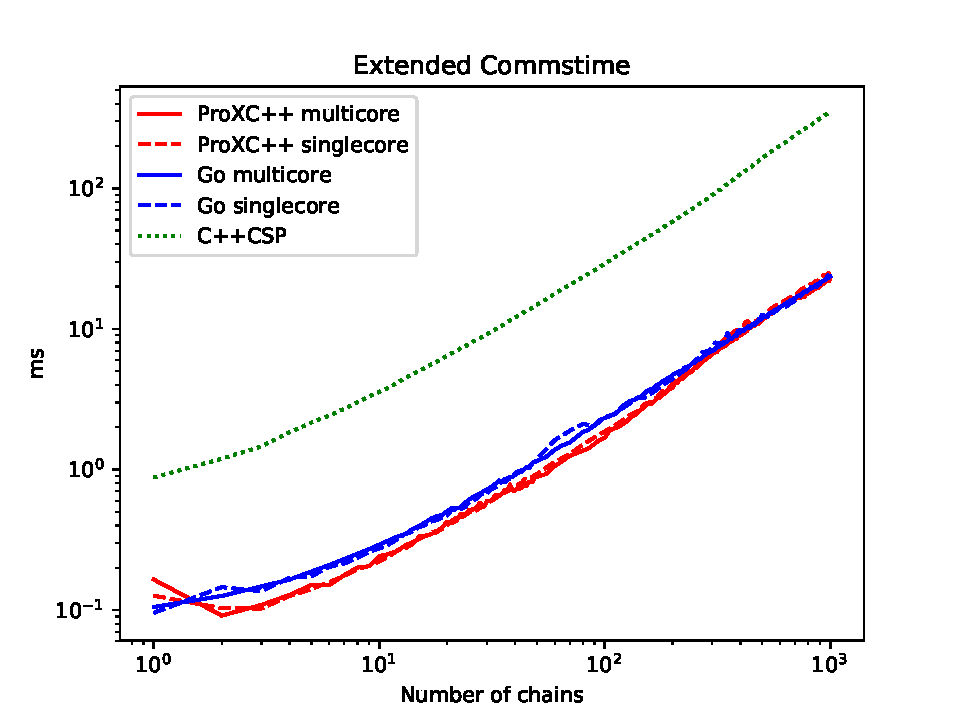
\includegraphics[width=0.9\linewidth]{fig/extended_commstime}
    \caption{Results of extended commstime. The Y axis has a logarithmic scaling.}
    \label{fig:extended_commstime}
\end{figure}


\FloatBarrier
%%%%%%%%%%%%%%%%%%%%%%%%%%%%%%%%%%%%%%%%
\subsection{Concurrent Mandelbrot}
\label{subsec:concurrent_mandelbrot_test}


Some problems are embarrassingly parallel \citep{wilkinson1999parallel}, where little to no effort is needed to separate the work load into parallel tasks. The Mandelbrot set is a perfect example of an embarrassingly parallel problem, where each point in the set can be calculated independently of each other.

Generating a Mandelbrot set is perfect for testing the parallel capabilities of the entries, such as how good the load balancing is.

For this benchmark, the Mandelbrot set is computed in the domain $x\in[-2.1;1.0]$ and $y\in[-1.3;1.3]$ with a resolution of a given dimension $D$. The set is split into $D$ number of lines on the Y axis, where each line consists of $D$ points evenly distributed along the X axis. Each line represents some parallel unit of work.

All lines are computed in a map\hyp{}reduce manner, where some worker processes each calculates a full line at a time. Two approaches will be tested: a hard coded optimal distribution of work, and dynamic sub\hyp{}optimal distribution of work.

Both approaches tests for the same; for a given dimension from $D=1$ to $1000$, how long does it take to calculate all lines, averaged over $100$ rounds. 

The hard coded optimal distribution is implemented by having the number of worker processes equal to the number of logical cores, $8$ in this case. Each worker process receives a line to calculate from a channel, where a producer process is on the other end continuously sending new lines to calculate. A consumer process receives finished calculated lines on a channel from the worker processes.

Note that for the singlecore version, only $1$ worker process is spawned as only a single core is available.

The results for the hard coded Mandelbrot test are presented in \cref{fig:mandelbrot_hardcoded}.

\begin{figure}[h!]
    \centering
    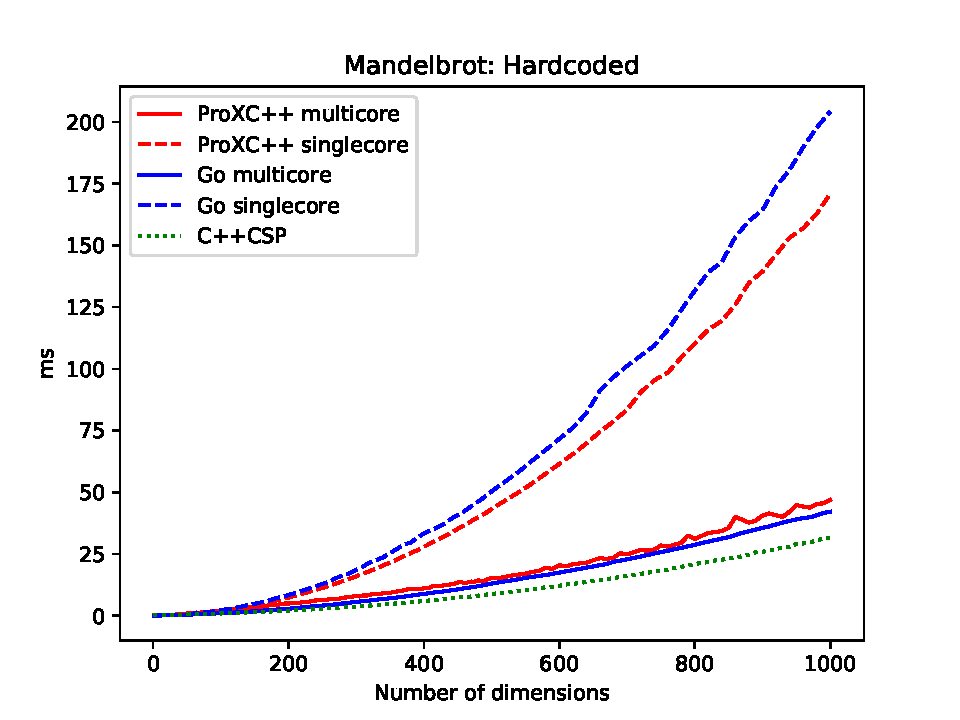
\includegraphics[width=0.9\linewidth]{fig/mandelbrot_hardcoded}
    \caption{Results of concurrent Mandelbrot with hard coded number of workers.}
    \label{fig:mandelbrot_hardcoded}
\end{figure}

The dynamic sub-optimal distribution is implemented by having worker processes each dedicated for calculating a single line, meaning a total of $D$ worker processes will be spawned for a dimension $D$. All worker processes will be spawned simultaneously. At consumer process will receive finished calculated lines on a channel from the worker processes, just as the hard coded Mandelbrot test.

The results for the dynamic Mandelbrot test are presented in \cref{fig:mandelbrot_dynamic}.  

\begin{figure}[h!]
    \centering
    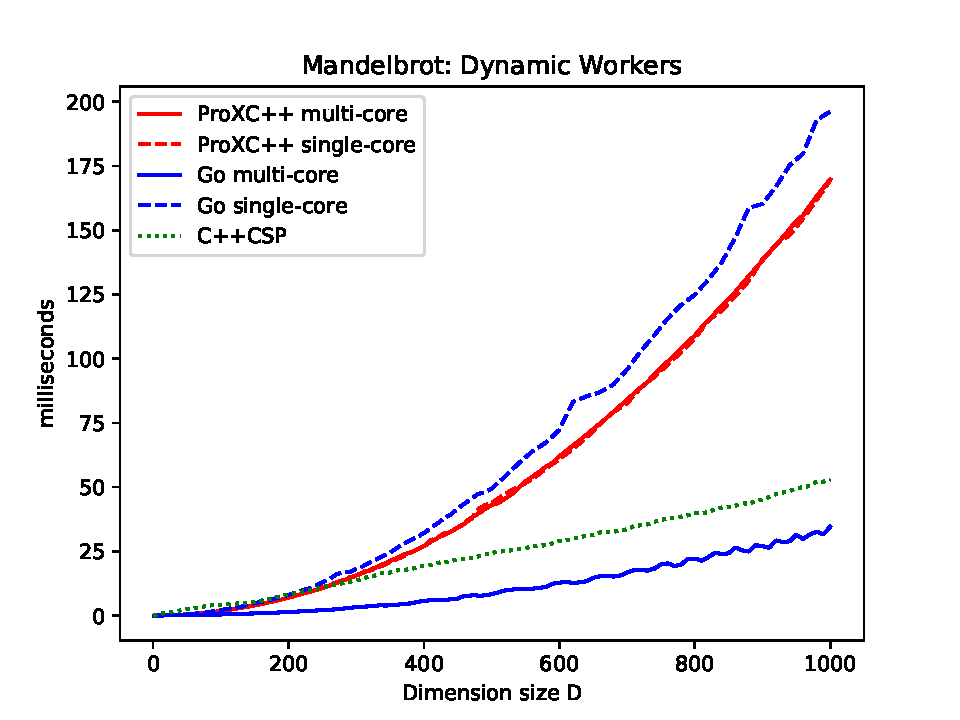
\includegraphics[width=0.9\linewidth]{fig/mandelbrot_dynamic}
    \caption{Results of concurrent Mandelbrot with dynamic number of workers.}
    \label{fig:mandelbrot_dynamic}
\end{figure}


\FloatBarrier
%%%%%%%%%%%%%%%%%%%%%%%%%%%%%%%%%%%%%%%%
\subsection{Concurrent Prime Sieve}


The last benchmark is the concurrent prime sieve, popularized by the famously elegant piece of concurrent code in Go \citep{go2017primesieve}. A prime sieve is a fast type of algorithm to find prime numbers, usually implemented as a sequential algorithm. A concurrent prime sieve is also an algorithm to find prime numbers, however daisy\hyp{}chains processes to determine whether a number is a prime or not. 

At the start of the daisy\hyp{}chain is the \textit{generator} process, which generates all numbers from $2$ and above. Along the daisy\hyp{}chain is \textit{filters} processes, where each filter represents a prime number along the number line. When the filter receives a number, the divisibility of that number is checked against the filters prime number. A non\hyp{}divisible number is passed along the daisy\hyp{}chain, while a divisible number is discarded. Given a daisy\hyp{}chain of $N$ filters, at the end of the daisy\hyp{}chain is the $N$th prime.

Note that the concurrent prime sieve algorithm is nowhere near as efficient as the sequential counterpart. The interesting merits of the concurrent prime sieve algorithm is however the total concurrent throughput. As multiple integers can be pipelined simultaneously in the daisy\hyp{}chain, it is possible to sieve multiple integers in parallel.

This benchmark test generates $N$ prime numbers, where $N=10$ to $1000$. Given a $N$, the execution time per prime number is calculated over the average running time of $10$ runs.

The results for the concurrent prime sieve test are presented in \cref{fig:concurrent_sieve}.

\begin{figure}[h!]
    \centering
    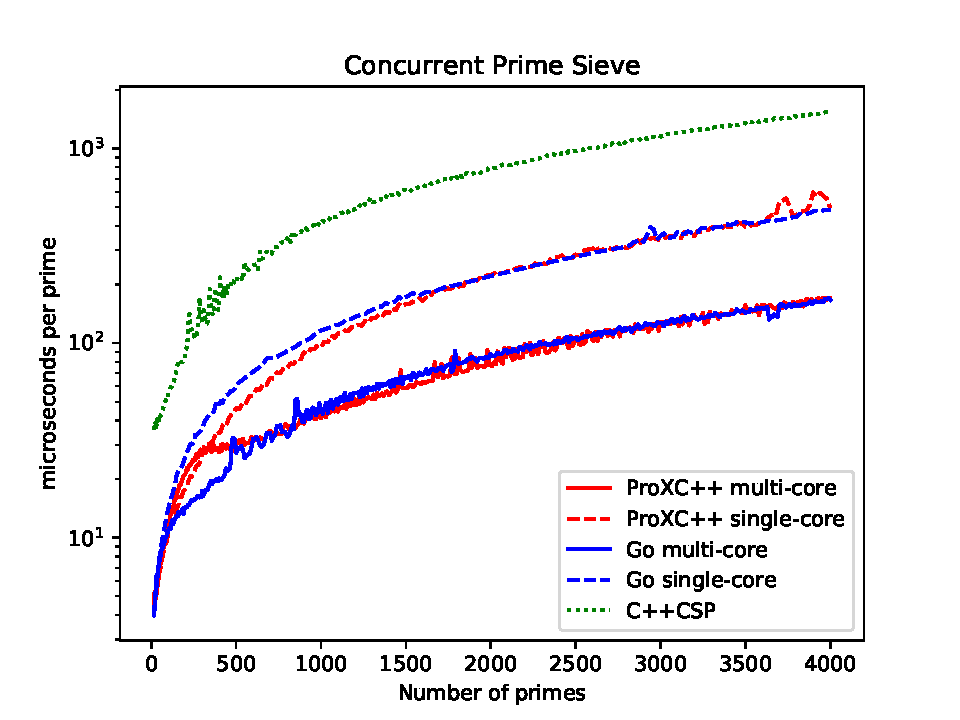
\includegraphics[width=0.9\linewidth]{fig/concurrent_sieve}
    \caption{Results of concurrent prime sieve. The Y axis has a logarithmic scaling.}
    \label{fig:concurrent_sieve}
\end{figure}


\FloatBarrier
%%%%%%%%%%%%%%%%%%%%%%%%%%%%%%%%%%%%%%%%%%%%%%%%%%%%%%%%%%%%%%%%%%%%%%%%%%%%%%%%
\section{Analysis}
\label{sec:analysis}


Starting with the extended commstime test, the results in \cref{fig:extended_commstime} shows both multicore and singlecore versions \Proxc{} and Go equals in execution time. A small exception is \Proxc{} being slightly faster than Go in the range $n\in[1;\sim{}300]$. As the chain length increases, both \Proxc{} and Go converges to a fixed execution time per chain, showing a linear increase in total execution time. 

The singlecore versions of both entries was expected to be the fastest, as extended commstime is nothing but a long sequential dependent cycle of processes. That both multicore versions matches, and sometimes surpasses, the singlecore versions is a good result. C++CSP behaves very similar to \Proxc{} and Go, however at a very much worse execution time per chain. 

The results of the hard coded Mandelbrot test in \cref{fig:mandelbrot_hardcoded} were interesting, but expected. The multicore and singlecore versions of both \Proxc{} and Go respectively increase in execution time with the same exponential trend. The singlecore version was expected to perform worst, while the multicore versions was expected to have a much better execution time. What is surprising is C++CSP being the best entry here. When thinking about it, C++CSP does have the most optimal setup here. Since each worker process in C++CSP is a kernel\hyp{}thread, each thread can run independently of each other on each core. Considering C++CSP is the best possible outcome, both multicore version of C++CSP and \Proxc{} yields a decent result.

The results of the dynamic Mandelbrot test in \cref{fig:mandelbrot_dynamic} however shows a different side. The same trends for the singlecore versions can be observed. C++CSP slightly doubles in execution time, while Go almost matches the results of the hard coded Mandelbrot test for C++CSP. The big surprise is now multicore \Proxc{} equals singlecore \Proxc{}. Further inspections of the running test processor utilization reveals the runtime system only fully utilizes a single processor core. What is happening is when the worker processes are spawned, everyone is placed on the same ready queue on the same parent scheduler. All other idle schedulers fail to effectively steal work of the one parent scheduler, resulting in only one scheduler having work to run. This test clearly highlights that \Proxc{} has issues with effectively distributing a huge number of small work across the idle schedulers.

Lastly, the results of the concurrent prime sieve test in \cref{fig:concurrent_sieve} are probably the most promising results. Fully utilizing the parallel nature in the concurrent prime sieve algorithm is very unintuitive, and heavily relies on the runtime system to detect ready work and effectively distribute said work among idle schedulers. The results show that the singlecore and multicore versions of \Proxc{} and Go both follow the same trend, where the multicore versions yields a much better result than the singlecore versions. C++CSP is a lot slower than the singlecore versions of \Proxc{} and Go, showing the lack of concurrent throughput in C++CSP. 

An interesting observation to make is between the prime range $n\in[1;\sim{}500]$ \Proxc{} is a great deal slower than Go until it suddenly drop to equal. A possible explanation is not able to effectively distribute the ready work as the processes are too short lived, sort of similar to the same issue withe the dynamic Mandelbrot test. However, over a certain limit around $\sim{}500$ processes the schedulers are able to steal the processes.



%%%%%%%%%%%%%%%%%%%%%%%%%%%%%%%%%%%%%%%%
\part{Discussions} \label{part:discussions}

% !TEX encoding = UTF-8 Unicode
%!TEX root = main.tex
% !TEX spellcheck = en-US
%%=========================================


%%%%%%%%%%%%%%%%%%%%%%%%%%%%%%%%%%%%%%%%%%%%%%%%%%%%%%%%%%%%%%%%%%%%%%%%%%%%%%%%%%%%%%%%%%
\chapter{\Proxc{} vs. ProXC}
\label{ch:proxc++_vs_proxc}
% single-core vs multi-core
% performance?
% ergonomics?
% feature difference, why some was chosen or not
% why some features?

As \Proxc{} is a continuation of the project ProXC \citep{pettersen2016proxc}, it is interesting to see the different design choices and capabilities the two projects exhibits.

This chapter compares and discusses the differences between the two projects \Proxc{} and ProXC, which includes differences such as abstractions, library features, usability, and performance. This comparison should provide an insightful look into both libraries, as both cater to the same motivation; providing a CSP abstraction for a programming language with no native support for CSP\hyp{}based concurrency.


%%%%%%%%%%%%%%%%%%%%%%%%%%%%%%%%%%%%%%%%%%%%%%%%%%%%%%%%%%%%%%%%%%%%%%%%%%%%%%%%
\section{Similarities and Differences}


\Cref{tab:library_features_comparison} gives a rough comparison between \Proxc{} and ProXC. The main difference to take from the comparison is the more dynamic feature set \Proxc{} provides compared to the feature set of ProXC. In \Proxc{}, a dynamic number of processes can be spawned in parallel, a dynamic number of alternatives can be alted on, etc. This dynamic approach allows to create more flexible and less hard coded programs, and consequently creating more maintainable and expressive concurrent systems.

\begin{table}
    \centering
    \begin{tabular}{l|l|l}
    
        \ignore{empty} & 
        \multicolumn{1}{c|}{\textbf{\Proxc{}}} & 
        \multicolumn{1}{c}{\textbf{ProXC}} 
        
        \\ \hline
        
        \textbf{\begin{tabular}[c]{@{}l@{}}Target\\ langauge\end{tabular}} & 
        \begin{tabular}[c]{@{}l@{}}The \Cpp{} programming\\ language.\end{tabular} &
        \begin{tabular}[c]{@{}l@{}}The C programming\\ language.\end{tabular}
        
        \\ \hline
        
        \textbf{\begin{tabular}[c]{@{}l@{}}Lightweight\\ processes\end{tabular}} & 
        \begin{tabular}[c]{@{}l@{}}Third party library, portable,\\ customizable stack types.\end{tabular} &
        \begin{tabular}[c]{@{}l@{}}Handwritten, not portable,\\ hard coded stack types.\end{tabular}
        
        \\ \hline
        
        \textbf{\begin{tabular}[c]{@{}l@{}}Process\\ spawning\end{tabular}} &
        \begin{tabular}[c]{@{}l@{}}Synchronous parallel \\ spawning of dynamic\\ number of processes.\end{tabular} &
        \begin{tabular}[c]{@{}l@{}}Synchronous/asynchronous\\ nested parallel and sequential\\ process spawning of\\ fixed number of processes.\end{tabular}
        
        \\ \hline
        
        \textbf{Channels} &
        \begin{tabular}[c]{@{}l@{}}Synchronous and unbuffered,\\ unidirectional, one-to-one, \\ type safe.\end{tabular} &
        \begin{tabular}[c]{@{}l@{}}Synchronous and unbuffered,\\ bidirectional, any-to-any,\\ size safe.\end{tabular}
        
        \\ \hline
        
        \textbf{Alternation} &
        \begin{tabular}[c]{@{}l@{}}Alting on dynamic number \\ of alternatives. Alternatives\\ include channel send and\\ receive, timeouts and skip.\end{tabular} &
        \begin{tabular}[c]{@{}l@{}}Alting on fixed number\\ of alternatives. Alternatives\\ include channel receive,\\ timeouts and skip.\end{tabular}
        
        \\ \hline
        
        \textbf{\begin{tabular}[c]{@{}l@{}}Threading\\ model\end{tabular}} &
        \begin{tabular}[c]{@{}l@{}}M:N, hybrid threading model.\\ Support for multi\hyp{}core.\end{tabular} &
        \begin{tabular}[c]{@{}l@{}}M:1, user threading model.\\ No support for multi\hyp{}core.\end{tabular}                                                      
    \end{tabular}
    \caption{Comparison of library specification and features between \Proxc{} and ProXC}
    \label{tab:library_features_comparison}
\end{table}


%%%%%%%%%%%%%%%%%%%%%%%%%%%%%%%%%%%%%%%%%%%%%%%%%%%%%%%%%%%%%%%%%%%%%%%%%%%%%%%%
\section{Various Capabilities}


A big difference between the two is the threading model used, where \Proxc{} uses a hybrid threading model while ProXC uses a user threading model. The use of threading models only affects the performance in concurrent programs. The same concurrent program running on both \Proxc{} and ProXC should behave just the same. However, since the main development in processor architectures is in multi\hyp{}core, there is an incentive to use the available resources for a potential performance gain.

Now, not everything is about performance. Some might argue correct and expressive abstractions are more important than performance. The abstractions available in \Proxc{} and ProXC are both based on CSP. However, \Proxc{} has a greater expressive power than ProXC because of replicators for parallel spawning and alternatives for alting. Due to this limitation, ProXC cannot express a dynamic numbers of processes and alternatives for alting.


%%%%%%%%%%%%%%%%%%%%%%%%%%%%%%%%%%%%%%%%%%%%%%%%%%%%%%%%%%%%%%%%%%%%%%%%%%%%%%%%
\chapter{Challenges with a Multi\hyp{}Core Library}
\label{ch:difficulty_multicore_csp}
% is performance important?
% using spinlocks vs other locks? hybrids?
% locking kernel-threads to cores

Creating a dynamic multithreaded CSP library for multi\hyp{}core architectures is mostly motivated by the potential performance increase in concurrent systems by utilizing the available cores. CSP is about creating a correct and expressive abstraction over concurrent systems rather than performance, but it is tempting to fully utilize multi\hyp{}core architectures because of the inherently parallel nature of CSP. Therefore, the rhetorical question is as follows: is the difficulty of implementing a dynamic multithreaded CSP library worth it?


%%%%%%%%%%%%%%%%%%%%%%%%%%%%%%%%%%%%%%%%%%%%%%%%%%%%%%%%%%%%%%%%%%%%%%%%%%%%%%%%
\section{Critical Sections}


What separates a single\hyp{}core vs. a multi\hyp{}core implementation of a user\hyp{}threaded runtime system is the ability with single\hyp{}core runtime systems to reason and control which states processes are in, when they are running, etc. This reasoning is especially important in critical regions of the runtime system, being able to justify certain states in algorithms based on process states.

For a single\hyp{}core runtime system, any critical regions and side effects can be fully reasoned about. Since only one process runs at any given moment, code running between descheduling points essentially becomes a mutual exclusion. Multicore runtime systems cannot follow the same reasoning, since it has much less control whether a given process is currently running on another processor core not. Critical regions in the runtime system must most likely enforce some sort of mutual exclusion. 


%%%%%%%%%%%%%%%%%%%%%%%%%%%%%%%%%%%%%%%%%%%%%%%%%%%%%%%%%%%%%%%%%%%%%%%%%%%%%%%%
\section{Choice of Mutual Exclusion Locks}


What kind of locks a multi\hyp{}core runtime system uses to enforce mutual exclusion is also important. Different locks and their variations, such as OS mutexes, spinlocks, read\hyp{}write locks, and so forth have a different impact on performance in different situations. For instance, given a lock is held for are short\hyp{}term held, then spinlocks are preferred. For locks with high contention, meaning multiple actors are trying to acquire the lock simultaneously, some type of non\hyp{}linear back off procedure is needed. Either way, choosing what kind of lock is suitable for a given situation requires knowledge of different locks and the situation itself.


%%%%%%%%%%%%%%%%%%%%%%%%%%%%%%%%%%%%%%%%%%%%%%%%%%%%%%%%%%%%%%%%%%%%%%%%%%%%%%%%
\section{Non\hyp{}Blocking vs Mutual Exclusion Design}


Sometimes, it is desirable to design a non\hyp{}blocking design rather than mutual exclusion design. A non\hyp{}blocking design is usually much more demanding to develop than a mutual exclusion design, as it is harder to prove the design is correct. Non\hyp{}blocking design is often preferable over mutual exclusion, as it both scales better with a number of processor cores and has a better throughput, but does have a higher latency per operation wise compared to mutual exclusion.


%%%%%%%%%%%%%%%%%%%%%%%%%%%%%%%%%%%%%%%%%%%%%%%%%%%%%%%%%%%%%%%%%%%%%%%%%%%%%%%%
\section{Pinning Kernel\hyp{}Threads to Processor Cores}


Multi\hyp{}core runtime systems must resort to some sort of schedulers, each running on a kernel\hyp{}thread. A factor to consider is whether to set thread affinity for each kernel\hyp{}thread, i.e. pinning each kernel\hyp{}thread to a different processor core. The idea is to avoid the operating system from migrating kernel\hyp{}threads between processor cores, which causes discrepancies in the runtime system. The counter argument is the operating system can help with load balancing kernel\hyp{}threads, when for instance a scheduler with a high work load runs on a less used processor core.


%%%%%%%%%%%%%%%%%%%%%%%%%%%%%%%%%%%%%%%%%%%%%%%%%%%%%%%%%%%%%%%%%%%%%%%%%%%%%%%%
\chapter{Shortcomings and Limitations}
\label{ch:shortcomings_limitations}


Much of the shortcomings and limitations present in ProXC has been improved upon in \Proxc{}, which includes enforcing correct usage and the portability issues with the user\hyp{}thread implementation. However, some issues are present in the current state of \Proxc{}.


%%%%%%%%%%%%%%%%%%%%%%%%%%%%%%%%%%%%%%%%%%%%%%%%%%%%%%%%%%%%%%%%%%%%%%%%%%%%%%%%
\section{Enforcing Correct Usage}


\Proxc{} goes to great lengths to enforce correct usage by using much of the semantic facilities present in the \Cpp{} programming language. However, all problems existing in \Cpp{} programs, such as null pointer dereferencing and memory leaks, are possible in \Proxc{} programs.  

It is impossible to create a system which always generates and enforces correct program behaviour, and somewhere does the line have to be drawn. For instance, channels in \Proxc{} are one\hyp{}to\hyp{}one, and if multiple processes where to operate on the same channel end simultaneously, the result would be undefined behaviour. Channel ends have therefore been made non\hyp{}copyable to enforce the channel end only having a single owner and user. It is however very easy to bypass this by sending a reference of the channel end when spawning a new process, making multiple users still possible. Having shared memory between processes is also entirely possible, but is highly discouraged.

\Proxc{} is all about providing a safe framework for creating concurrent systems. Creating a complete safe framework is impossible, as the foundation of \Cpp{} is inherently unsafe. Therefore, \Proxc{} only enforces correct usage to some degree, and let the rest be up to the programmer.


%%%%%%%%%%%%%%%%%%%%%%%%%%%%%%%%%%%%%%%%%%%%%%%%%%%%%%%%%%%%%%%%%%%%%%%%%%%%%%%%
\section{Inefficient Load Balancing}


\Proxc{} uses work stealing for load balancing work between schedulers. A scheduler continues to run work as long as it has ready work. However, when a scheduler runs out of work and becomes idle, it tries to steal ready work from other schedulers. How these idle schedulers decide when to steal, how much ready work to steal, and so forth is not optimal nor efficient.

Currently, when a scheduler becomes idle it tries to steal once from a random scheduler. If the steal is successful it resumes the stolen work. However, if the steal fails the scheduler sleeps for $1$ millisecond and tries again when it wakes up. There is no coordination between the schedulers, as a scheduler with lots of ready work has no way to indicate to other schedulers to steal from it. 

This sort of brute\hyp{}force approach to find ready work is of course not desirable, as a concurrent program with few parallel tasks will generate lots of unnecessary wake\hyp{}ups of from idle scheduler trying to find work. This periodical wake\hyp{}up can also cause unnecessary migration of tasks between schedulers when few sequential dependent tasks are running, which was highlighted in the concurrent Mandelbrot test in \cref{subsec:concurrent_mandelbrot_test}.

The unnecessary migration of tasks and wasteful wake\hyp{}ups becomes negligible after an amount of parallel semi\hyp{}independent tasks is surpassed in the program.


%%%%%%%%%%%%%%%%%%%%%%%%%%%%%%%%%%%%%%%%%%%%%%%%%%%%%%%%%%%%%%%%%%%%%%%%%%%%%%%%
\section{Wasteful use of Resources}


The \Proxc{} runtime system has to manage a great lot of resources, including user\hyp{}thread management and inter\hyp{}process communication. Much of the resources used with user\hyp{}thread management are one\hyp{}time use, meaning nothing is reused of stack or control data structures related to the user\hyp{}threads. This one\hyp{}time use creates lots of unnecessary allocations of dynamic memory which could have been reused for later use.

A smarter runtime system could detect these one\hyp{}time use resources and reuse the resource rather than deallocating them. This, of course, requires a much more complex resource management by the runtime system, and could potentially introduce a greater overhead.


%%%%%%%%%%%%%%%%%%%%%%%%%%%%%%%%%%%%%%%%%%%%%%%%%%%%%%%%%%%%%%%%%%%%%%%%%%%%%%%%
\section{Determinism and Real\hyp{}Time Characteristics}


An important selling point of CSP is the ability to reason how deterministic a CSP model is, usually via refining the model against a specification model. The very same attribute, determinism, is also important in real\hyp{}time systems. A real\hyp{}time system is where the time it takes to complete an operation is just as important as the result of the operation, and can have direct consequences of the system functionality.

The question is whether \Proxc{} qualifies to be used for any real\hyp{}time requirements. The abstractions provided by \Proxc{} are very much deterministic, except for alting. Alting uses a pseudo\hyp{}random distribution to choose an alternative when multiple alternatives are ready. The reasoning behind using a pseudo\hyp{}random distribution is it favours fairness over determinism.

Another factor of determinism in \Proxc{}, which is unrelated to CSP, is dynamic multithreading. As the runtime schedulers rely on work stealing for distributing parallel work, the deterministic characteristic of the runtime system is affected. An idle scheduler chooses its victim by random, which consequently makes a process being stolen or not random. If a time critical operation relies on certain processes to be distributed among the schedulers to meet its deadline, it is inherently non\hyp{}deterministic whether the deadline is met or not.


% !TEX encoding = UTF-8 Unicode
%!TEX root = main.tex
% !TEX spellcheck = en-US
%%=========================================


%%%%%%%%%%%%%%%%%%%%%%%%%%%%%%%%%%%%%%%%%%%%%%%%%%%%%%%%%%%%%%%%%%%%%%%%%%%%%%%%
\chapter{Future Work}
\label{ch:future_work}

There are some opportunities for future work for which the library could benefit from. This chapter discusses the biggest potential contenders for future work, which has been detected during the project time line.


%%%%%%%%%%%%%%%%%%%%%%%%%%%%%%%%%%%%%%%%%%%%%%%%%%%%%%%%%%%%%%%%%%%%%%%%%%%%%%%%
\section{More Efficient Runtime System}

The desire for an efficient runtime system is a no\hyp{}brainer. An optimal library would be as efficient as possible, but is rarely the case. There are however some aspects of the current implementation of the ProXC++ runtime system that can be directly addressed as inefficient or suboptimal, which could potentially increase the performance and processor utilization.

First, the work\hyp{}stealing protocol the schedulers use is not working properly. Ready work is not properly being distributed if the type of work is short lived or rarely deschedules. Schedulers are also inefficient at finding ready work if they are idle. Currently, when a scheduler tries to steal work and fails, it sleeps for $1$ millisecond and tries again. This is obviously not a good approach, as this generates unnecessary CPU time. Therefore, the work stealing protocol between schedulers has a huge improvement.

Secondly, allocation of processes and process stacks could be improved. Currently, nothing is reused when destroying a process after returning. Stack allocations could be pooled, which is supported by the Boost Context library. 

Lastly, the alt\hyp{}to\hyp{}alt synchronization between an alting channel send and alting channel receive is horribly inefficient. This has mostly to do with a poor design of two alting processes selecting each other. 


%%%%%%%%%%%%%%%%%%%%%%%%%%%%%%%%%%%%%%%%%%%%%%%%%%%%%%%%%%%%%%%%%%%%%%%%%%%%%%%%
\section{C Wrapper API}

ProXC++ is first of all a C++ library. It would however be interesting and potentially useful be able to use ProXC++ for C code as well. This would require to create a C wrapper API for ProXC++.

Now, why is it desirable to using ProXC++ in C code when ProXC is readily available for creating CSP programs in C? The main arguments are ProXC++ is portable and has multicore support, both of which would be much more challenging to achieve with ProXC. 

The biggest hurdle of creating a C wrapper API would be translating C++ semantics to C. ProXC++ uses a great amount such as templates and move semantics to enforce both type safety, generalized processes, and unique ownership of channel ends. Such semantics have no intuitive translation, and a more restrictive, generalized wrapper API has to probably be created to work in C.


%%%%%%%%%%%%%%%%%%%%%%%%%%%%%%%%%%%%%%%%%%%%%%%%%%%%%%%%%%%%%%%%%%%%%%%%%%%%%%%%
\section{Improving on the Library Feature Set}
% extended Tx/Rx
% Async I/O, networking
% class defined processes

The feature set provided by ProXC++ is a good foundation for creating any type of concurrent program with CSP abstractions. However, some library features could potentially be a good extension to the current feature set.

Extended channel input or output, also called extended rendezvous, is about extending the synchronization in channel sending and receiving. An extended rendezvous allows the sender or receiver to perform additional operations after the channel transmission has occured, but before both channel ends resumes execution. One could see this as a an ``invisible'' middle\hyp{}man process performing some operation without breaking the existing synchronization.

Class defined processes, same as in C++CSP2, could be an useful addition. Defining a process from a class point of view rather than a function allows for more rigid definitions of processes. A well defined constructor, destructor and execution body can be defined, as well a more intuitive syntax can be used, i.e. calling a class constructor rather than a process creation function.

Asynchronous I/O operations is not supported with ProXC++. Any call to a blocking system call effectively blocks the entire kernel\hyp{}thread, halting any progress of processes residing on the given kernel\hyp{}thread. Go has support for asynchronous I/O operations, letting a scheduler with its processes continue on another kernel\hyp{}thread while the blocking process halts the current kernel\hyp{}thread. Asynchronous I/O could be used to implement support for networking and other blocking operations, but would require extensive development of the current implementation.


% !TEX encoding = UTF-8 Unicode
%!TEX root = main.tex
% !TEX spellcheck = en-US
%%=========================================

\chapter{Conclusion}
\label{ch:conclusion}

\section{Availability}


\section{Acknowledgment}
% øyvind timers

%%%%%%%%%%%%%%%%%%%%%%%%%%%%%%%%%%%%%%%%
% appendices
\appendix
%!TEX root = main.tex
% !TEX spellcheck = en-US
%%=========================================

\chapter{Acronyms}

\begin{table}[h!]
    \centering
    \begin{tabular}{ll}
        \texttt{API}  & Application Programming Interface \\
        \texttt{CSP}  & Communicating Sequential Processes \\
        \texttt{FIFO} & First In, First Out \\
        \texttt{KRoC} & Kent Retargetable occam Compiler \\
        \texttt{HW}   & Hardware \\
        \texttt{ILP}  & Instruction-Level Parallelism \\
        \texttt{MPMC} & Multiple\hyp{}producer\hyp{}multiple\hyp{}consumer \\
        \texttt{MPSC} & Multiple\hyp{}producer\hyp{}single\hyp{}consumer \\
        \texttt{OS}   & Operating System \\
        \texttt{SPMC} & Single\hyp{}producer\hyp{}multiple\hyp{}consumer \\
        \texttt{SPoC} & Southampton's Portable occam Compiler \\
        \texttt{SPSC} & Single\hyp{}producer\hyp{}single\hyp{}consumer \\
        \texttt{SW}   & Software \\
        \texttt{TLS}  & Thread-Local Storage
    \end{tabular}
\end{table}
%!TEX root = main.tex
% !TEX spellcheck = en-US
%%=========================================


%%%%%%%%%%%%%%%%%%%%%%%%%%%%%%%%%%%%%%%%%%%%%%%%%%%%%%%%%%%%%%%%%%%%%%%%%%%%%%%%
\chapter{Listing of Benchmark Code}
\label{ch:benchmark_code}

%%%%%%%%%%%%%%%%%%%%%%%%%%%%%%%%%%%%%%%%%%%%%%%%%%%%%%%%%%%%%%%%%%%%%%%%%%%%%%%%
\section*{Extended Commstime}

%%%%%%%%%%%%%%%%%%%%%%%%%%%%%%%%%%%%%%%%
\subsection*{ProXC++}
\lstinputlisting[style=CustomC++]{code/proxc_commstime.cpp}

%%%%%%%%%%%%%%%%%%%%%%%%%%%%%%%%%%%%%%%%
\subsection*{Go}
\lstinputlisting[style=CustomGo]{code/go_commstime.go}

%%%%%%%%%%%%%%%%%%%%%%%%%%%%%%%%%%%%%%%%
\subsection*{C++CSP}
\lstinputlisting[style=CustomC++]{code/cppcsp_commstime.cpp}

%%%%%%%%%%%%%%%%%%%%%%%%%%%%%%%%%%%%%%%%%%%%%%%%%%%%%%%%%%%%%%%%%%%%%%%%%%%%%%%%
\section*{Concurrent Mandelbrot -- Hard Coded}

%%%%%%%%%%%%%%%%%%%%%%%%%%%%%%%%%%%%%%%%
\subsection*{ProXC++}
\lstinputlisting[style=CustomC++]{code/proxc_mandelbrot_hardcode.cpp}

%%%%%%%%%%%%%%%%%%%%%%%%%%%%%%%%%%%%%%%%
\subsection*{Go}
\lstinputlisting[style=CustomGo]{code/go_mandelbrot_hardcoded.go}

%%%%%%%%%%%%%%%%%%%%%%%%%%%%%%%%%%%%%%%%
\subsection*{C++CSP}
\lstinputlisting[style=CustomC++]{code/cppcsp_mandelbrot_hardcode.cpp}


%%%%%%%%%%%%%%%%%%%%%%%%%%%%%%%%%%%%%%%%%%%%%%%%%%%%%%%%%%%%%%%%%%%%%%%%%%%%%%%%
\section*{Concurrent Mandelbrot -- Dynamic}

%%%%%%%%%%%%%%%%%%%%%%%%%%%%%%%%%%%%%%%%
\subsection*{ProXC++}
\lstinputlisting[style=CustomC++]{code/proxc_mandelbrot_dynamic.cpp}

%%%%%%%%%%%%%%%%%%%%%%%%%%%%%%%%%%%%%%%%
\subsection*{Go}
\lstinputlisting[style=CustomGo]{code/go_mandelbrot_dynamic.go}

%%%%%%%%%%%%%%%%%%%%%%%%%%%%%%%%%%%%%%%%
\subsection*{C++CSP}
\lstinputlisting[style=CustomC++]{code/cppcsp_mandelbrot_dynamic.cpp}


%%%%%%%%%%%%%%%%%%%%%%%%%%%%%%%%%%%%%%%%%%%%%%%%%%%%%%%%%%%%%%%%%%%%%%%%%%%%%%%%
\section*{Concurrent Prime Sieve}

%%%%%%%%%%%%%%%%%%%%%%%%%%%%%%%%%%%%%%%%
\subsection*{ProXC++}
\lstinputlisting[style=CustomC++]{code/proxc_sieve.cpp}

%%%%%%%%%%%%%%%%%%%%%%%%%%%%%%%%%%%%%%%%
\subsection*{Go}
\lstinputlisting[style=CustomGo]{code/go_sieve.go}

%%%%%%%%%%%%%%%%%%%%%%%%%%%%%%%%%%%%%%%%
\subsection*{C++CSP}
\lstinputlisting[style=CustomC++]{code/cppcsp_sieve.cpp}


% glossaries
%\printglossary

% bibliography
\bibliographystyle{unsrtnat}
\addcontentsline{toc}{chapter}{\bibname}
\bibliography{library/refs}  

\end{document}
